% ---------------------------------------------------------------------------------------------------------------
% TEMPLATE EM LATEX PARA TRABALHO DE CONCLUSÃO DE CURSO DA URI ERECHIM
% (ESTE TEMPLATE NÃO É UM PROJETO OFICIAL DA URI) CONSULTE SEU ORIETADOR CASO QUEIRA UTILIZA-LO
% Este template foi baseado no template da Universidade Tecnológica Federal do Paraná UTFPR
%
% Template baseado no projeto: http://tcc.tsi.gp.utfpr.edu.br/paginas/modelos-latex-da-utfpr
%
%----------------------------------------------------------------------------------------------------------------
% Codificação: UTF-8
% LaTeX:  abnTeX2
% ---------------------------------------------------------------------------------------------------------------


% CARREGA CLASSE PERSONALIZADA COM AS NORMAS DA URI-----------------------------------------------------------
\documentclass[oneside]{template-config/uri-abntex2} %oneside -> impressão apenas frente

% INCLUI ARQUIVOS DE CONFIGURAÇÕES-------------------------------------------------------------------------------
% REFERÊNCIAS------------------------------------------------------------------
\usepackage[%
    alf,
    abnt-emphasize=bf,
    bibjustif,
    recuo=0cm,
    abnt-url-package=url,       % Utiliza o pacote url
    abnt-refinfo=yes,           % Utiliza o estilo bibliográfico abnt-refinfo
    abnt-etal-cite=3,
    abnt-etal-list=3,
    abnt-thesis-year=final
]{abntex2cite}                  % Configura as citações bibliográficas conforme a norma ABNT

% PACOTES----------------------------------------------------------------------
\usepackage[utf8]{inputenc}                                 % Codificação do documento
\usepackage[T1]{fontenc}                                    % Seleção de código de fonte
\usepackage{booktabs}                                       % Réguas horizontais em tabelas
\usepackage{color, colortbl}                                % Controle das cores
\usepackage{float}                                          % Necessário para tabelas/figuras em ambiente multi-colunas
\usepackage{graphicx}                                       % Inclusão de gráficos e figuras
\usepackage{icomma}                                         % Uso de vírgulas em expressões matemáticas
\usepackage{indentfirst}                                    % Indenta o primeiro parágrafo de cada seção
\usepackage{microtype}                                      % Melhora a justificação do documento
\usepackage{multirow, array}                                % Permite tabelas com múltiplas linhas e colunas
\usepackage{subeqnarray}                                    % Permite subnumeração de equações
\usepackage{lastpage}                                       % Para encontrar última página do documento
\usepackage{verbatim}                                       % Permite apresentar texto tal como escrito no documento, ainda que sejam comandos Latex
\usepackage{amsfonts, amssymb, amsmath}                     % Fontes e símbolos matemáticos
\usepackage[algoruled, portuguese]{algorithm2e}             % Permite escrever algoritmos em português
%\usepackage[scaled]{helvet}                                % Usa a fonte Helvetica
\usepackage{times}                                          % Usa a fonte Times
%\usepackage{palatino}                                      % Usa a fonte Palatino
%\usepackage{lmodern}                                       % Usa a fonte Latin Modern
\usepackage[bottom]{footmisc}                               % Mantém as notas de rodapé sempre na mesma posição
\usepackage{ae, aecompl}                                    % Fontes de alta qualidade
\usepackage{latexsym}                                       % Símbolos matemáticos
\usepackage{lscape}                                         % Permite páginas em modo "paisagem"
%\usepackage{picinpar}                                      % Dispor imagens em parágrafos
%\usepackage{scalefnt}
\usepackage{setspace}                                    % Permite redimensionar tamanho da fonte
%\usepackage{subfig}                                        % Posicionamento de figuras
%\usepackage{upgreek}                                       % Fonte letras gregas

% Redefine a fonte para uma fonte similar a Arial (fonte Helvetica)
% \renewcommand*\familydefault{\sfdefault}
% Configura todo o documento para times new roman
\renewcommand{\familydefault}{ptm}

\documentclass{scrreprt}
\makeatletter
\usepackage{color}
\definecolor{lightgray}{rgb}{0.95, 0.95, 0.95}
\definecolor{darkgray}{rgb}{0.4, 0.4, 0.4}
%\definecolor{purple}{rgb}{0.65, 0.12, 0.82}
\definecolor{editorGray}{rgb}{0.95, 0.95, 0.95}
\definecolor{editorOcher}{rgb}{1, 0.5, 0} % #FF7F00 -> rgb(239, 169, 0)
\definecolor{editorGreen}{rgb}{0, 0.5, 0} % #007C00 -> rgb(0, 124, 0)
\definecolor{orange}{rgb}{1,0.45,0.13}		
\definecolor{olive}{rgb}{0.17,0.59,0.20}
\definecolor{brown}{rgb}{0.69,0.31,0.31}
\definecolor{purple}{rgb}{0.38,0.18,0.81}
\definecolor{lightblue}{rgb}{0.1,0.57,0.7}
\definecolor{lightred}{rgb}{1,0.4,0.5}
\usepackage{upquote}
\usepackage{listings}
% CSS
\lstdefinelanguage{CSS}{
  keywords={color,background-image:,margin,padding,font,weight,display,position,top,left,right,bottom,list,style,border,size,white,space,min,width, transition:, transform:, transition-property, transition-duration, transition-timing-function},	
  sensitive=true,
  morecomment=[l]{//},
  morecomment=[s]{/*}{*/},
  morestring=[b]',
  morestring=[b]",
  alsoletter={:},
  alsodigit={-}
}

% JavaScript
\lstdefinelanguage{JavaScript}{
  morekeywords={typeof, new, true, false, catch, function, return, null, catch, switch, var, if, in, while, do, else, case, break},
  morecomment=[s]{/*}{*/},
  morecomment=[l]//,
  morestring=[b]",
  morestring=[b]'
}

\lstdefinelanguage{HTML5}{
  language=html,
  sensitive=true,	
  alsoletter={<>=-},	
  morecomment=[s]{<!-}{-->},
  tag=[s],
  otherkeywords={
  % General
  >,
  % Standard tags
	<!DOCTYPE,
  </html, <html, <head, <title, </title, <style, </style, <link, </head, <meta, />,
	% body
	</body, <body,
	% Divs
	</div, <div, </div>, 
	% Paragraphs
	</p, <p, </p>,
	% scripts
	</script, <script,
  % More tags...
  <canvas, /canvas>, <svg, <rect, <animateTransform, </rect>, </svg>, <video, <source, <iframe, </iframe>, </video>, <image, </image>, <header, </header, <article, </article
  },
  ndkeywords={
  % General
  =,
  % HTML attributes
  charset=, src=, id=, width=, height=, style=, type=, rel=, href=,
  % SVG attributes
  fill=, attributeName=, begin=, dur=, from=, to=, poster=, controls=, x=, y=, repeatCount=, xlink:href=,
  % properties
  margin:, padding:, background-image:, border:, top:, left:, position:, width:, height:, margin-top:, margin-bottom:, font-size:, line-height:,
	% CSS3 properties
  transform:, -moz-transform:, -webkit-transform:,
  animation:, -webkit-animation:,
  transition:,  transition-duration:, transition-property:, transition-timing-function:,
  }
}

\lstdefinestyle{htmlcssjs} {%
  % General design
%  backgroundcolor=\color{editorGray},
  basicstyle={\footnotesize\ttfamily},   
  frame=b,
  % line-numbers
  xleftmargin={0.75cm},
  numbers=left,
  stepnumber=1,
  firstnumber=1,
  numberfirstline=true,	
  % Code design
  identifierstyle=\color{black},
  keywordstyle=\color{blue}\bfseries,
  ndkeywordstyle=\color{editorGreen}\bfseries,
  stringstyle=\color{editorOcher}\ttfamily,
  commentstyle=\color{brown}\ttfamily,
  % Code
  language=HTML5,
  alsolanguage=JavaScript,
  alsodigit={.:;},	
  tabsize=2,
  showtabs=false,
  showspaces=false,
  showstringspaces=false,
  extendedchars=true,
  breaklines=true,
  % German umlauts
  literate=%
  {Ö}{{\"O}}1
  {Ä}{{\"A}}1
  {Ü}{{\"U}}1
  {ß}{{\ss}}1
  {ü}{{\"u}}1
  {ä}{{\"a}}1
  {ö}{{\"o}}1
}
%
\lstdefinestyle{py} {%
language=python,
literate=%
*{0}{{{\color{lightred}0}}}1
{1}{{{\color{lightred}1}}}1
{2}{{{\color{lightred}2}}}1
{3}{{{\color{lightred}3}}}1
{4}{{{\color{lightred}4}}}1
{5}{{{\color{lightred}5}}}1
{6}{{{\color{lightred}6}}}1
{7}{{{\color{lightred}7}}}1
{8}{{{\color{lightred}8}}}1
{9}{{{\color{lightred}9}}}1,
basicstyle=\footnotesize\ttfamily, % Standardschrift
numbers=left,               % Ort der Zeilennummern
%numberstyle=\tiny,          % Stil der Zeilennummern
%stepnumber=2,               % Abstand zwischen den Zeilennummern
numbersep=5pt,              % Abstand der Nummern zum Text
tabsize=4,                  % Groesse von Tabs
extendedchars=true,         %
breaklines=true,            % Zeilen werden Umgebrochen
keywordstyle=\color{blue}\bfseries,
frame=b,
commentstyle=\color{brown}\itshape,
stringstyle=\color{editorOcher}\ttfamily, % Farbe der String
showspaces=false,           % Leerzeichen anzeigen ?
showtabs=false,             % Tabs anzeigen ?
xleftmargin=17pt,
framexleftmargin=17pt,
framexrightmargin=5pt,
framexbottommargin=4pt,
%backgroundcolor=\color{lightgray},
showstringspaces=false,      % Leerzeichen in Strings anzeigen ?
}%
%
\makeatother
% CONFIGURAÇÕES DE APARÊNCIA DO PDF FINAL--------------------------------------
\makeatletter
\hypersetup{%
    portuguese,
    colorlinks=true,   % true: "links" coloridos; false: "links" em caixas de texto
    linkcolor=black,    % Define cor dos "links" internos
    citecolor=black,    % Define cor dos "links" para as referências bibliográficas
    filecolor=black,    % Define cor dos "links" para arquivos
    urlcolor=black,     % Define a cor dos "hiperlinks"
    breaklinks=true,
    pdftitle={\@title},
    pdfauthor={\@author},
    pdfkeywords={abnt, latex, abntex, abntex2}
}
\makeatother

% ALTERA O ASPECTO DA COR AZUL--------------------------------------------------
\definecolor{blue}{RGB}{41,5,195}

% REDEFINIÇÃO DE LABELS---------------------------------------------------------
\renewcommand{\algorithmautorefname}{Algoritmo}
\def\equationautorefname~#1\null{Equa\c c\~ao~(#1)\null}

% CRIA ÍNDICE REMISSIVO---------------------------------------------------------
\makeindex

% HIFENIZAÇÃO DE PALAVRAS QUE NÃO ESTÃO NO DICIONÁRIO---------------------------
\hyphenation{%
    qua-dros-cha-ve
    Kat-sa-gge-los
}



% INCLUI ARQUIVOS DO TRABALHO DE CONCLUSÃO DE CURSO (PRÉ-TEXTUAIS, TEXTUAIS, PÓS-TEXTUAIS)-----------------------

% INSERE CAPA E FOLHA DE ROSTO
% CAPA---------------------------------------------------------------------------------------------------

% ORIENTAÇÕES GERAIS-------------------------------------------------------------------------------------
% Caso algum dos campos não se aplique ao seu trabalho, como por exemplo,
% se não houve coorientador, apenas deixe vazio.
% Exemplos: 
% \coorientador{}
% \departamento{}

% DADOS DO TRABALHO--------------------------------------------------------------------------------------
\titulo{Gerenciamento e Acompanhamento de Rotas de Entrega}
\titleabstract{Delivery Routes Management and Tracking}
\autor{Gabriel Paulo Capoan Cechet}
\autorcitacao{CECHET, Gabriel} % Sobrenome em maiúsculo
\local{ERECHIM - RS}
\data{2019}

% NATUREZA DO TRABALHO-----------------------------------------------------------------------------------
% Opções: 
% - Projeto de Conclusão de Curso (Disciplina de Projeto)
% - Trabalho de Conclusão de Curso (se for Graduação)
% - Dissertação (se for Mestrado)
% - Tese (se for Doutorado)
% - Projeto de Qualificação (se for Mestrado ou Doutorado)
\projeto{Trabalho de Conclusão de Curso}

% TÍTULO ACADÊMICO---------------------------------------------------------------------------------------
% Opções:
% - Bacharel ou Tecnólogo (Se a natureza for Trabalho de Conclusão de Curso)
% - Mestre (Se a natureza for Dissertação)
% - Doutor (Se a natureza for Tese)
% - Mestre ou Doutor (Se a natureza for Projeto de Qualificação)
\tituloAcademico{Bacharel}

% ÁREA DE CONCENTRAÇÃO E LINHA DE PESQUISA---------------------------------------------------------------
% Se a natureza for Trabalho de Conclusão de Curso, deixe ambos os campos vazios
% Se for programa de Pós-graduação, indique a área de concentração e a linha de pesquisa
\areaconcentracao{}
\linhapesquisa{}

% DADOS DA INSTITUIÇÃO-----------------------------------------------------------------------------------
% Se a natureza for Trabalho de Conclusão de Curso, coloque o nome do curso de graduação em "programa"
% Formato para o logo da Instituição: \logoinstituicao{<escala>}{<caminho/nome do arquivo>}
\instituicao{Universidade Regional Integrada do Alto Uruguai e das Missões Campus de Erechim}
\departamento{Departamento de Engenharias e Ciência da Computação}
\programa{Curso de Ciência da Computação}
\disciplina{Projeto de Conclusão de Curso}
%\logoinstituicao{0.2}{dados/figuras/logo-instituicao.png} 

% DADOS DOS ORIENTADORES---------------------------------------------------------------------------------
%Prof. Dr.
\orientador{Guilherme Afonso Madalozzo}
%\orientador[Orientadora:]{Nome da orientadora}
\instOrientador{Instituição do orientador}

\coorientador{Nome do coorientador}
%\coorientador[Coorientadora:]{Nome da coorientadora}
\instCoorientador{Instituição do coorientador}

% FOLHA DE ROSTO--------------------------------------------------------------------------------------------------------

% Os dados podem ser alterados em /text-elements/pre-textuais/capa.tex

% PROJETO DE CONCLUSÂO DE CURSO
% \preambulo{{\imprimirprojeto} elaborado e apresentado na disciplina de {\imprimirdisciplina}, Curso de {\imprimirprograma}, {\imprimirdepartamento} da {\imprimirinstituicao}.}

% TRABALHO DE CONCLUSÃO DE CURSO
\preambulo{{\imprimirprojeto} apresentado como requisito parcial à obtenção do grau de {\imprimirtituloAcademico}, {\imprimirdepartamento} da {\imprimirinstituicao}.}

% DISSERTAÇÃO DE MESTRADO
% \preambulo{{\imprimirprojeto} apresentada ao Programa de \mbox{Pós-graduação} da {\imprimirinstituicao}, como requisito parcial para obtenção do título de {\imprimirtituloAcademico}.}

% TESE DE DOUTORADO
% \preambulo{{\imprimirprojeto} apresentada ao Programa de \mbox{Pós-graduação} da {\imprimirinstituicao}, como requisito parcial para a obtenção do título de {\imprimirtituloAcademico}.}

% PROJETO DE QUALIFICAÇÃO DE MESTRADO OU DOUTORADO
%\preambulo{{\imprimirprojeto} apresentado ao Programa de \mbox{Pós-graduação} da {\imprimirinstituicao}, como requisito parcial para a obtenção do título de {\imprimirtituloAcademico}.}

% OBSERVAÇÕES-----------------------------------------------------------------------------------------------------------
% Altere este arquivo APENAS comentando as linhas que não se aplicam ao tipo de trabalho acadêmico desejado.

% \include{text-elements/pre-textuais/folha-aprovação}

\begin{document}

\pretextual
\imprimircapa                                               	           % Comando para imprimir Capa
\imprimirfolhaderosto{}                                     		   % Comando para imprimir Folha de rosto
% \imprimirfolhadeaprovacao
% INSERE ELEMENTOS PRÉ-TEXTUAIS
%% DEDICATÓRIA------------------------------------------------------------------

\renewcommand{\dedicatorianame}{DEDICATÓRIA}

\begin{dedicatoria}

Altere este texto inserindo a dedicatória do seu trabalho. 

\end{dedicatoria}
          			   % Dedicatória
% AGRADECIMENTOS--------------------------------------------------------------------------------

\begin{resumo}[AGRADECIMENTOS]
\begin{SingleSpacing}

A minha família Claudete, Gilmar e Samanta que nunca mediram esforços durante esta longa jornada, sempre estando ao meu lado, me apoiando e me corrigindo nos devidos momentos, permitindo que tudo isso acontecesse ao longa da minha vida e não somente nestes anos como universitário, mas em todos os momentos. Agradeço também minha namorada Andrielle, que sempre foi compreensível diante do tempo investido a este trabalho, me dando apoio e incentivo, além de estar sempre disponível para ajudar como possível ao longo do trabalho e aguentando meus assuntos tecnológicos entendiantes. Merecem agradecimento também os professores do curso de Ciência da Computação por todo o conhecimento, manifestação do caráter, confiança e ética da educação no processo de formação profissional. Também agradeço aos amigos e companheiros de trabalhos, de forma especial ao Prof. Dr. Guilherme Afonso Madalozzo por todo auxílio durante o desenvolvimento do trabalho. A todos que direta ou indiretamente fizeram parte da minha formação, o meu muito obrigado.

\end{SingleSpacing}
\end{resumo}        			   % Agradecimentos
%% EPÍGRAFE---------------------------------------------------------------------

\renewcommand{\epigraphname}{EPÍGRAFE}

\begin{epigrafe}

\textit{Eu denomino meu campo de Gestão do Conhecimento, mas você não pode gerenciar conhecimento. Ninguém pode. O que pode fazer - o que a empresa pode fazer - é gerenciar o ambiente que otimize o conhecimento.}
\\  \hspace*{\fill} (PRUSAK, Laurence, 1997)

\end{epigrafe}

% OBSERVAÇÕES------------------------------------------------------------------
% Altere o texto para inserir a epígrafe do seu trabalho
              			   % Epígrafe
% RESUMO--------------------------------------------------------------------------------

\begin{resumo}[RESUMO]
\begin{SingleSpacing}

% % Não altere esta seção do texto--------------------------------------------------------
% \imprimirautorcitacao. \imprimirtitulo. \imprimirdata. \pageref {LastPage} f. \imprimirprojeto\ – \imprimirprograma, \imprimirinstituicao. \imprimirlocal, \imprimirdata.\\
% %---------------------------------------------------------------------------------------

Devido a falta de tecnologia empregada ao ramo de transportes, mais especificamente aos \textit{motoboys}, que extraviam seu tempo organizando a prévia da rota a cada lote de entrega. Sabendo da importância de cada segundo do trabalho prestado por esses profissionais ao seu ofício, está sendo proposto uma aplicação \textit{web} para gerência de rotas, consumidas através de API de troca de dados (JSON), disponibilizada pelo sistema de pedidos já implantado na empresa, utilizando ferramentas como: Laravel e Google Maps Platform. \\

\textbf{Palavras-chave}: Laravel. Aplicação Web. Geolocalização. Heroku.

\end{SingleSpacing}
\end{resumo}             			   % Resumo em Português
% ABSTRACT--------------------------------------------------------------------------------

\begin{resumo}[ABSTRACT]
\begin{SingleSpacing}

% % Não altere esta seção do texto--------------------------------------------------------
% \imprimirautorcitacao. \imprimirtitleabstract. \imprimirdata. \pageref {LastPage} f. \imprimirprojeto\ – \imprimirprograma, \imprimirinstituicao. \imprimirlocal, \imprimirdata.\\
% %---------------------------------------------------------------------------------------

ABSTRACT \\

\textbf{Keywords}: Delivery. Geolocation. Google Maps. Web application.

\end{SingleSpacing}
\end{resumo}             		           % Resumo em Inglês
% Lista de Figuras----------------------------------------------------------------

\pdfbookmark[0]{\listfigurename}{lof}
\listoffigures*
\cleardoublepage

% OBSERVAÇÕES---------------------------------------------------------------------
% Este arquivo não precisa de ser alterado, pois a lista é gerada automaticamente.
   % Lista de Figuras
% LISTA DE QUADROS----------------------------------------------------------------

\renewcommand{\listofquadrosname}{LISTA DE QUADROS}

\pdfbookmark[0]{\listofquadrosname}{loq}
\listofquadros*
\cleardoublepage

% OBSERVAÇÕES---------------------------------------------------------------------
% Este arquivo não necessita de ser editado. A lista é gerada automaticamente.   % Lista de Quadros
% LISTA DE TABELAS-------------------------------------------------------------

\pdfbookmark[0]{\listtablename}{lot}
\listoftables*
\cleardoublepage

% OBSERVAÇÕES-------------------------------------------------------------------
% Este arquivo não precisa ser alterado, pois a lista é gerada automaticamente.
         		   % Lista de Tabelas
% LISTA DE ABREVIATURAS E SIGLAS----------------------------------------------------------

\begin{siglas}
    \item[3D] Computação Gráfica Tridimensional
    \item[3G] Terceira Geração de Padrões e Tecnologias de Telefonia Móvel
    \item[A-GPS] \textit{Assisted Global Positioning System}
    \item[AJAX] \textit{Asynchronous JavaScript and XML}
    \item[API] \textit{Application Programming Interface}
    \item[BSD] \textit{Berkeley Software Distribution}
    \item[CDMA] \textit{Code Division Multiple Access}
    \item[CGI] \textit{Common Gateway Interface}
    \item[CLI] \textit{Command Line Interfaces}
    \item[CPF] Cadastro de Pessoa Física
    \item[FI] \textit{Form Interpreter}
    \item[GB] Gigabyte
    \item[GIS] \textit{Geographic Information System}
    \item[GNU] \textit{General Public License}
    \item[GPRS] \textit{General Packet Radio Service}
    \item[GPS] \textit{Global Position System}
    \item[GSM] \textit{Global System for Mobile Communications}
    \item[HTML] \textit{HyperText Markup Language}
    \item[HTTP] \textit{Hypertext Transfer Protocol}
    \item[ID] \textit{Integrated Development Environment}
    \item[IMAP] \textit{Internet Message Access Protocol}
    \item[IP] \textit{Internet Protocol}
    \item[JS] \textit{JavaScript}
    \item[JSON] \textit{JavaScript Object Notation}
    \item[MB] Megabyte
    \item[MPM] \textit{Multi-Processing-Modules}
    \item[MVC] \textit{Model-View-Controller}
    \item[NNTP] \textit{Network News Transfer Protocol}
    \item[ORM] \textit{Object Relational Mapper}
    \item[OSDB] \textit{Open Source Database Benchmark}
    \item[PDV] Ponto De Vendas
    \item[PHP] \textit{Personal Home Page}
    \item[POP3] \textit{Post Office Protocol}
    \item[POSIX] \textit{Portable Operating System Interface}
    \item[PSR] PHP \textit{Standard Recommendation}
    \item[QR] \textit{Quick Response}
    \item[RDBMS] \textit{Relational Database Management Systems}
    \item[REST] \textit{Representational State Transfer}
    \item[SGBD] Sistemas de Gestão de Base de Dados
    \item[SNMP] \textit{Simple Network Management Protocol}
    \item[SOAP] \textit{Simple Object Access Protocol}
    \item[SSL] \textit{Secure Sockets Layer}
    \item[TTFF] Tempo de Localização Inicial
    \item[URL] \textit{Uniform Resource Locator}
    \item[URI] \textit{Uniform Resource Identifier}
    \item[W3C] \textit{World Wide Web Consortium}
    \item[XML] \textit{Extensible Markup Language}
\end{siglas}

% OBSERVAÇÕES-----------------------------------------------------------------------------
% Altere a lista acima para definir os acrônimos e siglas utilizados neste trabalho
          		   % Lista de Abreviaturas e Siglas
%% LISTA DE SÍMBOLOS------------------------------------------------------------

\begin{simbolos}
    \item[$ \Gamma $] Letra grega Gama
    \item[$ \lambda $] Comprimento de onda
    \item[$ \in $] Pertence
\end{simbolos}

% OBSERVAÇÕES-------------------------------------------------------------------
% Altere a lista acima para definir os símbolos utilizados no trabalho
        		   % Lista de Símbolos
\pdfbookmark[0]{\lstlistlistingname}{lol}
\lstlistoflistings
\cleardoublepage   % Lista de Algoritmos
% SUMÁRIO----------------------------------------------------------------------

\renewcommand{\contentsname}{SUMÁRIO}

\pdfbookmark[0]{\contentsname}{toc}
\tableofcontents*
\cleardoublepage               			   % Sumário

\textual
% INSERE ELEMENTOS TEXTUAIS
% INTRODUÇÃO-------------------------------------------------------------------

\chapter{INTRODUÇÃO}

Atualmente existem aplicações cruciais para facilitar a organização que um dia corrido necessita, como: lista de tarefas para você se lembrar de coisas que não podem ser esquecidas, GPS inteligente para guiar você sempre pelos melhores caminhos em sua cidade e previsão do tempo para nunca mais ser pego de surpresa na rua, são algumas funções de grande auxílio na vida de qualquer um. O princípio básico para desenvolvimento de uma aplicação é afirmar que um problema existe e precisa ser resolvido.

Locomoção é uma grande preocupação para quem vive em grandes centros urbanos. Utilizar o carro nem sempre é uma experiência agradável, afinal, não é nada difícil encontrar congestionamentos, principalmente quando é necessário atravessar a cidade para entregar ou buscar um objeto. É por esse motivo que a profissão chamada motoboy surgido provavelmente em São Paulo e disseminado em todo o país em 1998 \cite{MotoboyVeja}.

No cenário atual, é necessário uma otimização de rotas para estes profissionais da área de transportes que estão suscetíveis a perda de tempo caso não analisadas coerentemente por alguém capacitado. Um aplicativo móvel conectado a Google Maps Platform, proporcionando uma solução significativa na economia de tempo para os usuários.

Utilizando a Google Maps Platform, é possível encontrar o melhor trajeto até o destino com dados abrangentes e trânsito em tempo real. Oferecendo experiências personalizadas e ágeis que levam o mundo real até os usuários com mapas estáticos e dinâmicos. 

No segundo capítulo, são detalhadas as tecnologias utilizadas no desenvolvimento deste trabalho, como é o caso dos métodos de geolocalização disponíveis atualmente, o Sistema de Posicionamento Global Assistido (A-GPS) e o serviço de pesquisa e visualização de mapas e imagens de satélite da Terra gratuito na web Google Maps, fornecido pela Google.

O terceiro capítulo aborda o estudo das técnicas e ferramentas que foram necessárias para construção de toda a aplicação, passando pela linguagem base, servidor independente de plataforma, \textit{frameworks}, banco de dados e servidor web utilizados.

No quarto capítulo é descrito o desenvolvimento da aplicação Delivery Routes, assim como todos os passos realizados no decorrer do trabalho: captura dos dados, painel de gerenciamento para controle das entregas e o posterior acompanhamento das rotas de entregas.

Por fim, no quinto capítulo são apresentadas as conclusões e as propostas para futuros trabalhos.
% TECNOLOGIAS-------------------------------------------------------------------

\chapter{TECNOLOGIAS}
Neste capítulo estão descritas as tecnologias aplicadas no decorrer do trabalho.

\section{Geolocalização}
A geolocalização é capacidade de informar suas coordenadas e pode conseguir recuperar essas informações através do IP, GPS, conexão de \textit{Wi-Fi}, entre outros. Extremamente útil para uma serie de objetivos como informações sobre um determinado local ou uma rota de navegação, a API de geolocalização consiste em um método para localizar exatamente a posição de um usuário, simples de ser implementada e utilizada. Existem duas formas de realizar a captura da geolocalização através da API W3C, compatível com navegadores em \textit{desktop} ou dispositivos móveis. É necessária a autorização do usuário para acessar as suas informações de geolocalização, pois pode comprometer a sua privacidade e integridade \cite{geolocalizacao:2011}.

Compatibilidade com navegadores em \textit{desktop}:
\begin{itemize}
    \item Firefox 3.5 +;
    \item Chrome 5.0 +;
    \item Opera 10,60 +;
    \item Internet Explorer 9.0 +.
\end{itemize}

Compatibilidade com navegadores em dispositivos móveis:
\begin{itemize}
    \item Android 2.0 +;
    \item iPhone 3.0 +;
    \item Opera Mobile 10.1 +;
    \item Symbian (S60 3rd e 5 ª geração);
    \item Blackberry OS 6;
    \item Maemo;
\end{itemize}

\subsection{Fontes de geolocalização}
Para obter a localização do usuário, estão disponíveis várias fontes diferentes, tendo cada uma seu próprio grau de precisão e variação e precisão. Por intermédio do navegador instalado em um \textit{desktop} o sistema de geolocalização utiliza \textit{Wi-Fi} (precisão de 20 metros) ou o IP que só se faz necessário ao nível de cidade, podendo fornecer algumas vezes falsas informações. Por sua vez, os dispositivos móveis utilizam a técnica de triangulação do GPS (precisão de 10m), \textit{Wi-Fi} e GSM/CDMA celular com uma precisão de 1000 metros \cite{geolocalizacao:2011}.

\subsubsection{Métodos: getCurrentPosition e watchPosition}
Os dois métodos retornam imediatamente, e depois de forma assíncrona tentam obter a localização atual. Eles carregam o mesmo número de argumentos, dois deles são opcionais: um \textit{callback} quando retornar corretamente, um \textit{callback} se ocorrer erro, e um objeto \textit{PositionOptions}, que terão as seguintes opções:

\begin{itemize}
    \item enableHighAccuracy: indica se deseja receber os resultados mais precisos, podem ter respostas mais lentes, ele recebe um valor \textit{boolean};
    \item timeout: tempo que o dispositivo demora para retornar uma posição, recebe um valor em milissegundos, com o padrão de 0;
    \item maximumAge: denota o tempo máximo de uma posição em cache que o aplicativo estará disposto a aceitar. Tudo isso sendo realizado em milissegundos com o valor padrão 0, significando que uma tentativa deve ser realizada para obter um novo objeto imediatamente.
\end{itemize}

Para capturar a posição enquanto tiver alteração, como movimentação do disponível, é necessário utilizar o método \textit{watchPosition}, mantendo a informação sobre o código (para cancelar o monitoramento basta passar o id pra o método \textit{clearWatch}) e a mudança de posição, então basicamente mantém atualizada a posição do usuário, contendo dentro do bloco uma posição do objeto existem as propriedades presentes na \autoref{fig:figura-propertycoords}. Entre estes, apenas ''coords.latitude'' e ''coords.longitude'' são garantidos para serem devolvidos (todos os outros podem ser nulos) \cite{geolocalizacao:2011}.

\begin{figure}[H]
    \centering
    \caption{Propriedades dos métodos de geolocalização}
    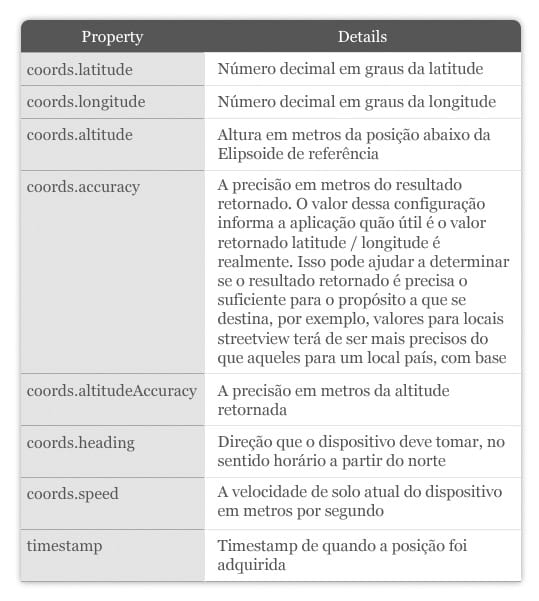
\includegraphics[width=0.8\textwidth]{./dados/figuras/fig1}
    \fonte{\cite{oficinanetagps:2018}}
    \label{fig:figura-propertycoords}
\end{figure}

\section{A-GPS}
A-GPS (\textit{Assisted Global Positioning System}), desenvolvida para localizar satélites com mais rapidez e confiabilidade, utiliza recursos de rede para localizar e utilizar os satélites em condições de sinal fraco. É uma versão otimizada do  GPS (\textit{Global Position System}), que recebe dados através de uma conexão de dados (GPRS ou 3G), permitindo que o aparelho calcule as coordenadas da sua posição atual ao receber informações satelitais, sob certas condições, como pode ser visto na \autoref{fig:figura-funcagps} \cite{oficinanetagps:2018}. 

\begin{figure}[H]
    \centering
    \caption{Funcionamento do A-GPS}
    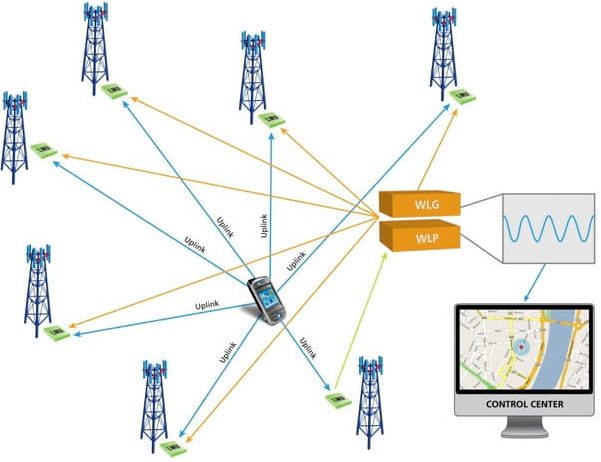
\includegraphics[width=1.0\textwidth]{./dados/figuras/fig2}
    \fonte{\cite{oficinanetagps:2018}}
    \label{fig:figura-funcagps}
\end{figure}

Esta tecnologia se torna superior a sua antecessora devido a precisão e disponibilidade das coordenadas do dispositivo em tempo real, apesar dos custos cobrados pela transferência de dados sobre a rede celular pela operadora utilizada, não sofrendo alterações de propagação \textit{multipath} (caminhos secundários que o sinal percorre até chegar à antena do receptor, como mostrado na \autoref{fig:figura-propagmultipath}), como por exemplo, de construções, ruas, edifícios, rios, lagos, veículos ou condições atmosféricas \cite{oficinanetagps:2018} \cite{multicaminho:2004}.

 A maior utilidade do sistema de A-GPS, se faz em áreas urbanas, repletas de desfiladeiros urbanos, melhorando a experiência do usuário para todos os aplicativos que usam o GPS integrado e reduzindo o tempo que um aparelho com GPS leva para localizar a sua posição atual, conhecido como TTFF (Tempo de Localização Inicial) \cite{oficinanetagps:2018}.

\begin{figure}[H]
    \centering
    \caption{O problema do multipath}
    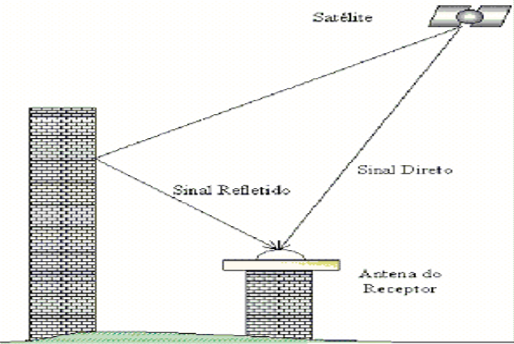
\includegraphics[width=0.8\textwidth]{./dados/figuras/fig3}
    \fonte{\cite{multicaminho:2004}}
    \label{fig:figura-propagmultipath}
\end{figure}

%\subsubsection{Diferenças entre GPS e A-GPS}
%\subsection{Propagação Multipath}

\section{Google Maps}
O Google Maps é um dos recursos da Google mais popular de todos, amplamente utilizado por aqueles que querem se garantir na hora de chegar a um local desconhecido. Além de oferecer o serviço de mapas, o software inclui outras características muito úteis, como ferramentas para calcular as direções entre dois pontos. Pode-se obter mais informações sobre qualquer lugar, graças à utilização de fotos, \textit{webcams} e artigos. Seja pelos seus recursos básicos, como encontrar endereços específicos e verificar trajetos e distâncias entre dois ou mais pontos, ou pelos avançados, como a visão de satélite e o Street View, ele se destaca com facilidade neste mercado. Em parte graças à sua enorme abrangência, poucas cidades e ruas ainda não estão nele, permitindo fazer o \textit{download} de uma área no dispositivo para ser usado sem conexão com a internet, através das áreas \textit{off-line}. Os mapas salvos dessa forma são renovados a cada 30 dias por meio de redes \textit{Wi-Fi}, caso o usuário fique mais de 30 dias sem usá-los, o aplicativo sugerirá que ele renove a área ou a apague para economizar espaço. Esse recurso é especialmente útil caso você viaje para outro país e não tenha plano de dados móveis \cite{google:2019}. Na \autoref{fig:figura-googlemaps} pode-se ver um exemplo de visualização de mapa do Google Maps.

\begin{figure}[H]
    \centering
    \caption{Exemplo de visualização do Google Maps}
    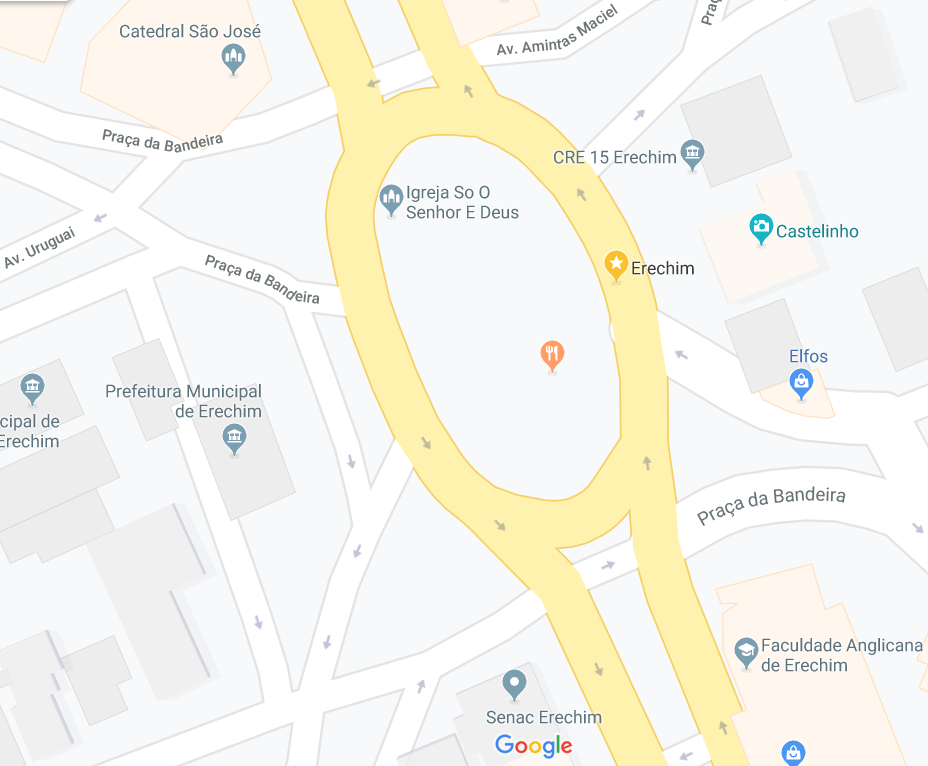
\includegraphics[width=0.9\textwidth]{./dados/figuras/fig4}
    \fonte{\cite{googleMaps:2019}}
    \label{fig:figura-googlemaps}
\end{figure}

A principal utilização é a busca por endereços, a partir de um computador, independentemente do navegador e do sistema operacional, basta digitar o endereço que deseja encontrar. Além de digitar o local manualmente, você pode indicá-lo diretamente no mapa. Também é possível descobrir novos locais, como lojas, restaurantes entre outros pontos de interesse facilmente, através de categorias e subcategorias, como “para ir com crianças” e “para gastar pouco”. Tudo isso, são locais escolhidos com base na localização atual e que se adaptam ao gosto de cada usuário. É comum ser disponibilizado mais de um caminho para o destino final, exibindo por padrão a mais rápida, levando em consideração a variação de trânsito para o horário atual. Isso é possível porque o Google Maps acumula informações sobre o tráfego da região. Ou seja, ele sabe qual é o fluxo de veículos para um determinado local em um determinado horário. Além de encontrar qualquer localidade, demonstrar informações meteorológicas ou indicações e caminhar ao redor das cidades mais importantes do globo, é um de seus diferenciais \cite{google:2019}.

Para ajudar quem andar de ônibus, metrô e trem pelas cidades do mundo, é possível saber a melhor rota de transporte público, qual o ponto de ônibus mais perto e os pontos de parada do coletivo. Dispondo de serviços de altitude para ciclistas, é possível identificar as variações do terreno em metros durante o trajeto, além de levar em conta a estrutura cicloviária da cidade. Às vezes, esse caminho pode nem ser o mais direto entre os dois pontos, mas ele pretende ser o mais seguro e agradável para quem está pedalando \cite{google:2019}.

Com uma enorme base de dados, serviços como Booking, Decolar ou Kayak, podem ser encontrados ao pesquisar por um hotel na plataforma da Google, contando com uma ferramenta interna para ajudar seus usuários, que apresentam diversas opções de quartos vagos na região, com o preço médio. Caso o local de visita escolhido durante uma viagem seja bem conhecido, é possível fazer um \textit{tour} pelo espaço interno mapeado. No Maracanâ, por exemplo, é possível visualizar a divisão das arquibancadas. O plano da empresa é estender esse recurso a outros estabelecimentos de grande porte, como parques e shoppings. Muitas das opções de uso citadas fazem parte da Google Street View, que mapeia locais possíveis de caminhar virtualmente por várias cidades ao redor do mundo, podendo encontrar exatamente a fachada do local desejado. Além do Google Earth e dos Indoor Maps, o Google Maps traz também outra função capaz explorar o mundo a partir da tela do computador chamada Google Treks, desenvolvido para visitar virtualmente alguns lugares incríveis da Terra.
Selecionando a cidade de partida e a cidade de chegada e o meio de transporte ''Avião'', faz o Google Maps exibir informações de voos disponíveis para o trajeto, é possível obter informações relacionadas a duração do voo e quais companhias aéreas operam aquele trajeto \cite{google:2019}. 

O recurso mais recente adicionado a plataforma, permite planejar uma rota com \textit{waypoints}, é a possibilidade de fazer percursos que incluam diversas parada, indicando o melhor caminho do ponto A até B, e depois de B até C, sem precisar mudar a rota novamente, muito usado para encontrar o melhor caminho para visitar diversos pontos turísticos de uma cidade no mesmo dia.

Várias ferramentas de visualização geoespacial dos principais \textit{players} da indústria da internet estão tomando o mundo digital. Google, Yahoo, Microsoft e Amazon lançaram ferramentas de mapeamento baseada em geolocalização e, coletivamente, elevaram o nível de mapeamento da internet. Por mais que suas capacidades funcionais não forneçam nada de muito diferente do que fornecedores tradicionais da GIS (\textit{Geographic Information System}) já tinham, o surgimento destes serviços foi significativo na medida em que conseguiram captar um público mais amplo. O Google entrou como líder destes serviços com seu produto Google Maps, que fornece uma interface visual atrativa, construídas com tecnologia AJAX, além de dados detalhados de imagens aéreas da superfície terrestre, e uma API aberta que permite a personalização do mapa, incluindo a capacidade de adicionar dados específicos ao mapa e traçar rotas \cite{geospatial:2009}.

\subsection{Google Maps Platform}
A plataforma para desenvolvedores da Google se chama Google Maps Platform, onde 99\%
de cobertura no mundo, abrangendo de mais de 200 países e territórios, estão disponíveis. Contemplando informações de local precisas e em tempo real, são mais de 25 milhões de atualizações por dia e 1 bilhão de usuários ativos por mês, tudo isso gerando uma grande base de dados para consulta \cite{google:2019}. Nela, se obtêm soluções para cada setor:
\begin{itemize}
    \item Serviço de transporte particular: disponibiliza a integração com qualquer aplicativo de serviço de transporte particular para diminuir os tempos de espera dos clientes e os erros de navegação dos motoristas;
    \item Jogos: permite criar jogos imersivos e realistas com milhões de estruturas em 3D personalizáveis, dados globais atualizados e integração perfeita com o Unity;
    \item Rastreamento de recursos: possibilita maior eficiência na localização de veículos e os recursos em tempo real, visualizando o trajeto dos mesmos e orientando os motoristas durante viagens complexas. 
\end{itemize}

\subsubsection{Maps}
O recurso Maps presente na Google Maps Platform, leva o mundo real até os usuários por meio de mapas estáticos e dinâmicos, imagens do Google Street View e visualizações 360º, visualizando o mundo com mapas eficientes e precisos, podendo ser incorporado em sites ou aplicativos. 

O Street View e as imagens de satélite de alta resolução permitem criar experiências mais atraentes com ainda mais detalhes, podendo trabalhar com personalizações e sobreposições de acordo como gosto do usuário. Capacidade, confiabilidade ou desempenho, não é um problema para a equipe Google, a infraestrutura está sempre disponível para ampliação \cite{google:2019}. 

\subsubsection{Routes}
Através de dados abrangentes e trânsito em tempo real, encontrar o melhor caminho até o destino final se torna um trabalho rápido com o uso do recurso Routes. Com informações de navegação confiáveis e mais de 64 milhões de quilômetros de estradas em todo o mundo, traçar percursos entre cidades ou encontrar hotéis, permite maior eficiência, redução de custos e melhorar a experiência dos clientes finais. Este recurso permite planejar viagens munido de dados atualizados sobre a distância entre pontos, trajetos sugeridos e tempos estimados de deslocamento, com a capacidade de criar trajetos eficientes para até 25 pontos de referência, agilizando os sistemas de entrega, criando itinerários para turistas ou guiar os clientes que alugam carros do seu escritório até os hotéis, realocando o mesmo caso o caminho escolhido possua tráfego \cite{google:2019}. Sua eficiência é justificada pelo agrupamento dos seguinte recursos:

\begin{itemize}
    \item Directions: fornece rotas de transporte público, bicicleta, carro e a pé, calcula os tempos de deslocamento atuais ou futuros com base no trânsito em tempo real;
    \item Distance Matrix: calcula tempos de deslocamento e distâncias para um ou mais locais;
    \item Roads: permite criar itinerários precisos determinando o trajeto percorrido pelo veículo e as vias mais próximas ao longo de cada ponto da viagem do veículo.
\end{itemize}

\subsubsection{Places}
Contempla informações avançadas de mais de 150 milhões de pontos de interesse, permitindo encontrar locais específicos por meio de números de telefone, endereços e sinais em tempo real. Com usuários atualizando a todo momento, 24 horas por dia, as avaliações medidas pela Google se tornam confiantes, capazes de planejar uma viagem ou indicar um restaurante através dos gostos dos usuários. Com o Places, é possível compartilhar detalhes sobre nomes de locais, endereços, classificações, comentários, dados de contato e ambiente. Os Local Guides e os usuários enviam milhões de atualizações todos os dias \cite{google:2019}. Este recurso é o maior agrupador de todos, abrange:

\begin{itemize}
    \item Place Details: fornece nomes, endereços e outros detalhes valiosos, como classificações, avaliações ou dados de contato de pontos de interesse;
    \item Current Place: identifica um local com base nos sinais em tempo real, como hora do dia ou local;
    \item Find Place: localiza usando o número de telefone, endereço ou nome do local;
    \item Preenchimento automático: sugere informações de local enquanto os usuários digitam;
    \item Geocoding: converte endereços em coordenadas geográficas e vice-versa;
    \item Geolocation: captura o local preciso de um dispositivo usando o \textit{Wi-Fi} ou torres de celular como base;
    \item Time Zone: mostra o fuso horário de qualquer local.
\end{itemize}
% FERRAMENTAS--------------------------------------------------------------------

\chapter{FERRAMENTAS}
Este Capítulo descreve as ferramentas utilizadas para desenvolvimento do presente trabalho.

%\section{Maps JavaScript API}

\section{PHP}
PHP é um acrônimo recursivo para PHP: \textit{Hypertext Preprocessor} (Pré-Processador de Hipertexto), que originalmente se chamava \textit{Personal Home Page} (Página Inicial Pessoal), é uma linguagem de \textit{script open source} de uso geral, muito utilizada, e especialmente adequada para o desenvolvimento web e que pode ser embutida dentro do HTML, segundo \citeonline{phpdevelopment}. O que distingue o PHP de algo como o JS no lado do cliente é que o código é executado no servidor, gerando o HTML que é então enviado para o navegador. O navegador recebe os resultados da execução desse \textit{script}, mas não sabe qual era o código fonte

\citeonline{bentodesenvolvimento} explica que PHP é uma ferramenta que possibilita o pré-processamento de páginas HTML. Dessa forma, PHP consegue alterar o conteúdo de uma página, antes de enviá-la para o navegador. Além disso, PHP também permite capturar entradas de dados do usuário, como formulários e outras formas de interação. Trata-se de uma linguagem altamente popular devido à sua natureza de código aberto e suas funcionalidades versáteis, sendo uma linguagem de \textit{script} do tipo \textit{server-side} com diversos propósitos. Porém, ela é principalmente utilizada para gerar conteúdos dinâmicos em um site.

Destaca-se do pensamento de \citeonline{bentodesenvolvimento}, existem diversos motivos para escolher esta tecnologia, alguns motivos são:

\begin{itemize}
    \item Nasceu para a web e sua integração com qualquer sistema operacional, banco de dados e servidor web é simples, mais baratos e fáceis de encontrar;
    \item Curva de aprendizado suave, comparada a outras linguagens;
    \item Tecnologia livre;
    \item Suporte para conversar com outros serviços usando protocolos como IMAP, POP3, HTTP.
\end{itemize}

Atualmente, o PHP, é uma das linguagens de programação mais usadas no mundo. O termo PHP foi criado com apenas um aglomerado de códigos CGI (elemento que torna a ligação física ou lógica entre dois sistemas ou servidores, descritos em uma linguagem C). A ideia inicial era acompanhar o tráfego do site pessoal do criador. Os anos passaram e o criador desenvolvia \textit{scripts}, o que aumentava os recursos que o site dele tinha \cite{phpdevelopment}.

Ainda conforme o autor citado acima, o sucesso dessa linguagem foi tão grande que o criador, Rasmus Lerdof, transformou o aglomerado de códigos CGI em uma linguagem de programação. Com isso, a grande maioria dos sites e aplicações passaram a utilizar o PHP como linguagem principal.

%IntegrandoPHPcomMySQL \cite{bentodesenvolvimento}

\section{Laravel}
Laravel é um \textit{framework} livre, de código aberto, voltado para desenvolvimento de sistemas baseado em internet e feito em PHP. Tem como principal característica auxiliar no desenvolvimento de aplicações seguras e performáticas de forma rápida, com código limpo e simples, já que ele incentiva o uso de boas práticas de programação e utiliza o padrão PSR-2 como guia para estilo de escrita do código. Foi criado por Taylor Otwell e tem como principal função desenvolver aplicações web com padrão de arquitetura MVC. Algumas características nativas do Laravel são: sua sintaxe descomplicada e concisa, um sistema modular com gerenciador de dependências dedicado, várias formas de acesso a banco de dados relacionais e vários utilitários indispensáveis no auxílio ao desenvolvimento e manutenção de sistemas. O código fonte do Laravel está hospedado no GitHub e licenciado sob os termos da licença MIT \cite{portalgsti:laravel}. 

Segundo \citeonline{locaweb:laravel}, Laravel é o \textit{framework} que está no top \textit{trends} dos mais buscados no Google, isso desde agosto de 2014, que coincide com o ano de lançamento da versão 5.0. Sua divisão em rotas, \textit{controllers} e \textit{models}, sendo compatível com diversos bancos de dados, trabalhando de forma relacional ou orientada a objetos como: MySQL, Postgress, Redis, MongoDB, Cassandra e SQL Server, utilizando \textit{features} Scaffold ou Internacionalização (i18n), faz com que o Laravel seja altamente compatível. Sendo assim, basta ajustar as configurações e definir qual o banco de dados desejado e o sistema mantém seu funcionamento caso a estrutura estiver pronta, utilizando uma implementação simples do ActiveRecord chamada de Eloquent ORM, que é uma ferramenta que traz várias funcionalidades para facilitar a inserção, atualização, busca e exclusão de registros. Para a criação de interface gráfica, o Laravel utiliza uma \textit{engine} de \textit{template} chamada Blade, que traz uma gama de ferramentas que ajudam a criar interfaces bonitas e funcionais de forma rápida e evitar a duplicação de código.

\begin{citacao}
 O Laravel é uma estrutura de aplicativos da web com sintaxe expressiva e elegante. Acreditamos que o desenvolvimento deve ser uma experiência agradável e criativa para ser verdadeiramente gratificante. O Laravel tenta aliviar a dor do desenvolvimento, facilitando tarefas comuns usadas na maioria dos projetos da web \cite{laravel}.
\end{citacao}

Com sua baixa curva de aprendizagem e elegância, seu diferencial é a grande quantidade de recursos nativos que o mesmo contém para auxiliar o processo de desenvolvimento. Além disso, o \textit{framework} tem como objetivo aumentar a velocidade de codificação, sem esquecer características importantes como a segurança e performance da aplicação.

Segundo \citeonline{comparisonLaravel}, afirmaram que ao comparar PHP procedural com CodeIgniter e Laravel, o Laravel tem bom desempenho e menos tempo de execução para todas as quatro ações. Os resultados em milissegundos de dez entradas como média para as quatro ações são apresentados na \autoref{tab:comparisonLaravel}.

\begin{table}[H]
    \centering
    \caption{Resultado do experimento no tempo de execução
    \label{tab:comparisonLaravel}}
    \begin{tabular}{rrrrr}
            \toprule
            & CREATE    & READ      & UPDATE    & DELETE \\
            \midrule
            PLAIN PHP   & 0.066     & 0.063    & 0.0925   & 0.065 \\
            CODEIGNITER & 0.0634    & 0.0747   & 0.0825   & 0.616 \\
            LARAVEL     & 0.201     & 0.222    & 0.312    & 0.301 \\
            \bottomrule
    \end{tabular}
    \fonte{\citeonline{comparisonLaravel}}
\end{table}

\citeonline{He2015/01} também prova a eficácia do método de projeto web com base na estrutura do Laravel, criando um ambiente operacional virtual e comparando com o mesmo ambiente desenvolvido em CodeIgniter. De acordo com a \autoref{fig:He2015/01}, a eficiência do desenvolvimento baseado em Laravel é maior em comparação com o método tradicional de design da web baseado na estrutura do CodeIgniter, justificado pela escalabilidade robusta, de modo a melhorar a eficiência do desenvolvimento.

\begin{figure}[H]
    \centering
    \caption{Tendências de eficiência de desenvolvimento - Laravel e CodeIgniter}
    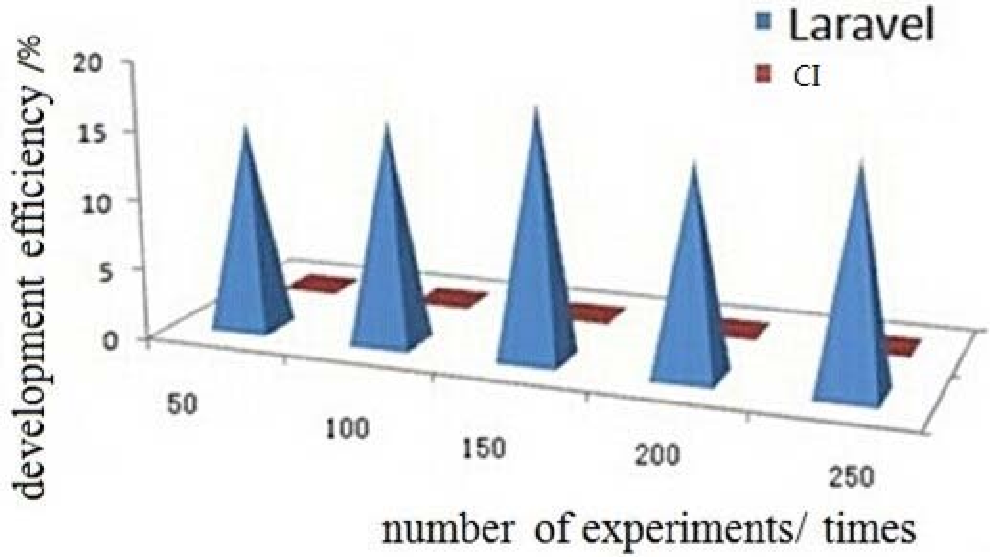
\includegraphics[width=0.6\textwidth]{./dados/figuras/fig9}
    \fonte{\citeonline{He2015/01}}
    \label{fig:He2015/01}
\end{figure}

%%%Para utilização do Laravel é preciso das ferramentas básicas para desenvolvimento em PHP, sugere-se: o XAMPP, pois já incluem o servidor Apache, banco de dados MySql e o próprio PHP, além disso será necessário realizar a instalação do Composer, através do qual é realizada a instalação do Laravel.

\section{Apache}
%Em 1995, Robert McCool e seu grupo de pesquisa desenvolveram o servidor web Apache. O nome originou-se de uma tribo indígena de mesmo nome. O Apache é um software livre, ou seja, possui um código aberto, distribuído sob a licença GNU, ou seja, é gratuito e pode ser estudado e modificado através de seu código fonte por qualquer pessoa. Além disso, é o servidor da web mais popular desde abril de 1996 \cite{netcraft}.

Segundo \citeonline{apache:webmedia}, o servidor web Apache é projetado para trabalhar com uma ampla variedade de plataformas e ambientes. Isto é possível devido à sua implementação  modular. Introduzindo modelos de processos MPM (Multi-Processing-Modules), responsáveis por gerenciar as portas de comunicação, aceitar conexões e alocar processos ou \textit{threads} para atendimento das requisições.

Como \citeonline{apache:Marcelo} fala em seu artigo, o Apache é \textit{open source}, multi-plataforma mais utilizado em todo o mundo. As principais características do Apache são flexibilidade, altamente configurável, robustez, escalabilidade, pode ser configurado para diferentes funções e é composto de módulos separados onde cada um implementa uma característica diferente.

\citeonline{apache:magazine} comenta em uma edição da revista Infra Magazine que a excelência desta aplicação e a qualidade que um software \textit{open source} pode obter quando possui um desenvolvimento maduro e sério. O principal fator relacionado à performance é o número de instâncias do servidor. O Apache suporta um grande número de instâncias simultâneas, onde cada uma é relacionada a um cliente acessando o servidor, oferecendo também suporte a módulos que, quando instalados, adicionam funcionalidades ao servidor. Como exemplos, pode-se citar o \textit{mod\_php}, \textit{mod\_python}, \textit{mod\_ftp}, entre outros, o que permite que os usuários escrevam seus próprios módulos por meio da API do software.

O Apache é composto por módulos (\autoref{fig:modularizacaoApache}) para segurança, cache, reescrita de URL, autenticação de senhas e mais. O módulo denominado de \textit{mod\_ssl} por exemplo, adiciona a capacidade do servidor de atender solicitações usando o protocolo HTTPS. Este protocolo faz uso da camada SSL para a criptografia de todos os dados transferidos, proporcionando maior segurança entre o tráfego de dados entre cliente e servidor,  disponibilizado para Windows, Novell Netware, OS/2 e outros sistemas do padrão POSIX, como o Unix e o Linux, onde é amplamente utilizado \cite{apache:magazine}.

\begin{figure}[H]
    \centering
    \caption{Modularização Apache}
    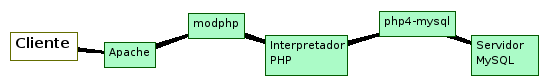
\includegraphics[width=0.9\textwidth]{./dados/figuras/fig12}
    \fonte{\citeonline{modapache}}
    \label{fig:modularizacaoApache}
\end{figure}

%%% Por exemplo, quando você acessa uma página em PHP em um site que roda sobre um servidor Apache, ele (Apache) lê o arquivo no disco e repassa a requisição para o modphp, o módulo encarregado de processar arquivos PHP. Ele, por sua vez, aciona o interpretador PHP, que processa a página e a entrega, já processada, ao Apache, que, finalmente, a entrega ao cliente. Caso seja necessário acessar um banco de dados (como no caso de um fórum), entra em ação outro módulo, como o php4-mysql, que permite que o interpretador PHP acesse o banco de dados:

%https://canaltech.com.br/internet/O-que-e-servidor-Apache/
%https://www.hostinger.com.br/tutoriais/o-que-e-apache
%https://www.weblink.com.br/blog/o-que-e-apache

\section{MySQL}
%

%Acessandoeusandoumbancode dados \cite{bentodesenvolvimento}

%% REVISÃO DE LITERATURA--------------------------------------------------------

\chapter{REVISÃO DE LITERATURA}
\label{chap:fundamentacaoTeorica}

É uma boa prática iniciar cada novo capítulo com um breve texto introdutório (tipicamente, dois ou três parágrafos) que deve deixar claro o quê será discutido no capítulo, bem como a organização do capítulo.
Também servirá ao propósito de "amarrar"{} o conteúdo deste capítulo com o conteúdo do capítulo imediatamente anterior.
         
% DESENVOLVIMENTO DA APLICAÇÃO-------------------------------------------------------------------

\chapter{DESENVOLVIMENTO DA APLICAÇÃO}
%https://rafaell-lycan.com/2015/construindo-restful-api-laravel-parte-1/

%%% Rev-Madalozzo: Este parágrafo está ruim. Muito longo com poucas pausas. Não tem pontuação final nas frases, muitas vírgulas. Tenta refazer de uma maneira mais amigável para o leitor poder respirar :)
A proposta para este trabalho foi a construção de uma API REST que possibilita a coleta das coordenadas geográficas dos pedidos gerados no estabelecimento, juntamente com o desenvolvimento de uma aplicação encarregada de gerenciar os pedidos como entregas com um painel de controle para geração de lotes de entregas. Em conjunto com o módulo de entrega, destinado ao motoboy, no qual consegue observar, em um mapa, a rota e pontos de parada que devem ser percorridos, tudo isso em tempo real.

\section{Softwares utilizados}

Esta Seção apresenta os softwares utilizados na etapa de codificação da aplicação. Para diminuir o custo de desenvolvimento, optou-se pela utilização de tecnologias gratuitas. Outro importante ponto na escolha das ferramentas é a questão de documentação disponível na comunidade web.

\begin{itemize}
    \item PhpStorm: IDE completa de desenvolvimento para projetos codificados com a linguagem de programação PHP;
    \item Composer: gerenciador de pacotes em nível de aplicativo, que fornece um formato padrão para gerenciar dependências de software PHP e bibliotecas necessárias;
    \item Cmder: console para execução de linhas de comandos para o sistema operacional Windows. Com essa ferramenta é possível executar comandos Unix diretamente no Windows; %(\textit{ls}, \textit{rm}, \textit{mv} e etc)
    \item Laravel: \textit{framework} de programação baseada na linguagem PHP;
    \item Artisan CLI: interface de linha de comando incluída no Laravel, fornecendo vários comandos úteis durante a criação da aplicação, por exemplo: configuração de ambiente, verificar rotas, interagir com a aplicação e criar diversos tipos de arquivos (\textit{Migrations}, \textit{Controllers} e \textit{Models});
    \item Blade: ferramenta para criação de interfaces gráficas, utilizado pelo Laravel como uma ferramenta de \textit{template}, trazendo uma quantidade grande de funcionalidades que ajudam na criação de interfaces interativas;
    \item Eloquent ORM: ferramenta com funcionalidades que facilitam a inserção, atualização, busca e exclusão de registros diretamente no banco de dados;
    \item XAMPP: servidor independente de plataforma, que inclui: Apache, MySQL, phpMyAdmin, FileZilla FTP Server, OpenSSL, PHP e Perl;
    \item Jaspersoft Studio: ferramenta para projetar e executar modelos de relatório com expressões, gráficos, mapas, tabelas e \textit{QR Codes}, criando documentos de qualquer complexidade a partir de informações presentes no banco de dados;
    \item GitHub: plataforma de hospedagem de código-fonte para controle de versão;
    \item Sourcetree: representação visual de repositórios da nuvem.
\end{itemize}

\newpage
Para o desenvolvimento deste trabalho, foi escolhido trabalhar com Laravel 5.8.11, um \textit{framework} com um servidor interno já incluso e invocado através do comando \textit{php artisan serve}, em conjunto com o XAMPP, um servidor independente de plataforma para executar sistemas localmente, que consiste principalmente na base de dados MySQL e os interpretadores para linguagens de \textit{script}: PHP e Perl, o que facilita e agiliza o desenvolvimento. Como o conteúdo estará armazenado  na rede local, o acesso aos arquivos é realizado instantaneamente, ficando disponível no endereço \textit{http://127.0.0.1}.

A execução do comando \textit{composer create-project --prefer-dist laravel/laravel delivery-routes} no Cmder gera, de forma padronizada, toda a estrutura de um projeto Laravel, apresentada na \autoref{fig:base-projeto}. O uso do Cmder torna o desenvolvimento, via terminal, do sistema operacional Windows mais amigável. Uma vez que esta ferramenta possibilita a execução de comandos Unix em ambiente Microsoft.

\begin{figure}[H]
    \centering
    \caption{Estrutura Laravel}
    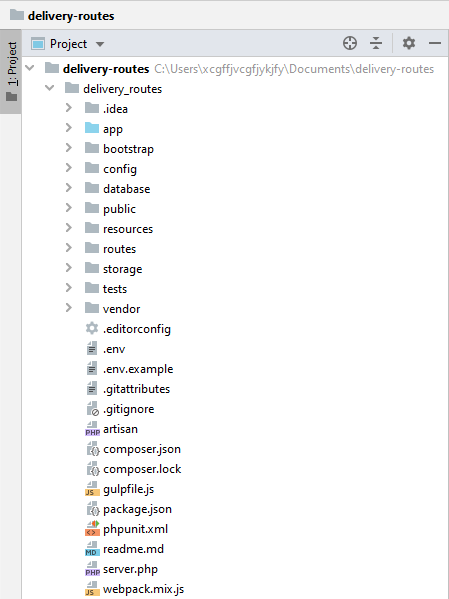
\includegraphics[width=0.5\textwidth]{./dados/figuras/fig6}
    \fonte{Autor}
    \label{fig:base-projeto}
\end{figure}

\newpage
Foi necessária uma série de configurações de ambiente para que se tornasse possível o desenvolvimento da aplicação: primeiramente foi preciso instalar e configurar todas as dependências do PHP para que se pudesse ter acesso a linguagem de programação através do gerenciados de dependências Composer. 

Foi optado, por questões de segurança, hospedar o código-fonte do projeto em nuvem, através da plataforma GitHub. A sincronia entre os arquivos locais e o GitHub foi possível com o auxílio do sistema de controle de versões chamado Git, representado visualmente pelo Sourcetree, que deixa o trabalho braçal por linha de comando (\textit{gitbash}) de lado, sendo também necessário sua instalação e configuração na máquina de desenvolvimento. 

O banco de dados escolhido para armazenar os registros foi o MySQL, cuja instalação e configuração ocorreu automaticamente pelo XAMPP. Por último, para ter acesso a manipulação do código, um editor de texto era necessário, optando-se pelo PHPStorm. Esta, uma IDE paga, mas utilizando o e-mail acadêmico da URI, obtive a licença estudantil, terminando assim a fase configuração de ambiente de desenvolvimento e garantindo aptidão para começar os trabalhos.

O próximo passo foi a modelagem dos dados, onde verificou-se que seria necessário a criação das seguintes tabelas com o recurso \textit{Migration}: \textit{users}, \textit{motoboys}, \textit{deliveries}, \textit{payments} e \textit{orders}. Uma sexta tabela chamada de \textit{deliveries\_orders} precisou ser criada para vincular mais de um pedido à cada entrega, onde uma \textit{trigger}, disparada via \textit{after update}, ficou responsável pela atualização do status de cada pedido vinculado à entrega, esta chamada de \textit{tr\_Status\_Orders}, apresentada no \autoref{alg:trigger}.

\begin{lstlisting}[caption={Trigger tr\_Status\_Orders}, label=alg:trigger, style=SQL]
CREATE TRIGGER tr_Status_Orders AFTER UPDATE ON `deliveries`
FOR EACH ROW BEGIN
    UPDATE `orders` o SET `status` = NEW.status WHERE `id` IN
        (SELECT `order_id` FROM `deliveries_orders`
        WHERE `delivery_id` = NEW.id); 
END
\end{lstlisting}

O recurso do Laravel chamado \textit{Migration}, é tem por objetivo gerenciar as mudanças estruturais do banco de dados da aplicação. Para cada tabela, coluna ou índice criados no banco de dados, é possível usar a \textit{migration} para fazer essa operação automática, visando organizar e definir uma sequência de criação das tabelas. Para aplicações com poucas tabelas a utilização de \textit{migrations} para gerenciar a estrutura das tabelas é extremamente útil e válida.

\newpage
\section{Módulo de gerenciamento}
 Inicialmente, o objetivo era construir uma aplicação completa para gestão de vendas, focando na geração do pedido e entrega, sendo essa para qualquer ramo de atividade. Porém descobriu-se a possibilidade de um nicho de mercado ainda não explorado e sem concorrentes, em que não é preciso disputar clientes com grandes empresas renomadas e maduras no assunto.
 
 A aplicação desenvolvida foca no gerenciamento das rotas de entregas dos pedidos gerados via e-PDV já operantes, necessitando apenas da disponibilização de uma API no formato de arquivo JSON (\autoref{fig:drHttpAPI}), essa compondo-se de dados essenciais para realização da integração automática abordada na próxima Seção.
 
  \begin{figure}[H]
    \centering
    \caption{Delivery Routes - Requisição HTTP}
    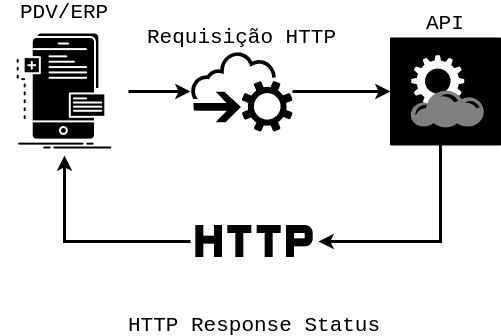
\includegraphics[width=0.6\textwidth]{./dados/figuras/fig16}
    \fonte{\citeonline{iFood}}
    \label{fig:drHttpAPI}
\end{figure}
 
 Primeiramente é preciso entender os possíveis status e o fluxo de um pedido integrado na Delivery Routes, ambos representados na \autoref{tab:drStatusPedido} e na \autoref{fig:drStatusPedido}.
 
 \begin{table}[H]
    \centering
    \caption{Delivery Routes - Status do pedido
    \label{tab:drStatusPedido}}
\begin{tabular}{|l|l|}
\hline
\textbf{Status} & \textbf{Descrição} \\ \hline
PLACED & Indica um pedido foi colocado no sistema. \\ \hline
CONFIRMED & Indica um pedido confirmado. \\ \hline
INTEGRATED & Indica um pedido que foi integrado no sistema. \\ \hline
CANCELLED & Indica um pedido que foi cancelado. \\ \hline
DISPATCHED & Indica um pedido que foi despachado ao cliente. \\ \hline
DELIVERED & Indica um pedido que foi entregue. \\ \hline
CONCLUDED & Indica um pedido que foi concluído. \\ \hline
\end{tabular}
    \fonte{\citeonline{iFood}}
\end{table}
 
 \begin{figure}[H]
    \centering
    \caption{Delivery Routes - Fluxo do status do pedido}
    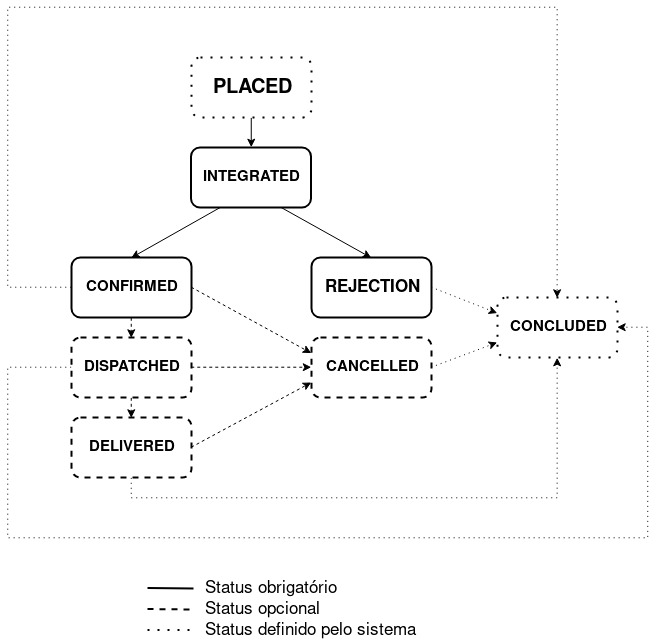
\includegraphics[width=0.6\textwidth]{./dados/figuras/fig15}
    \fonte{\citeonline{iFood}}
    \label{fig:drStatusPedido}
\end{figure}

%%%Se o valor da coluna token_access é diferente ao hash da sessão siginfica que o usuário fez um novo login e gerou um novo hash. Neste caso podemos deslogar o usuário, caso os valores não se coinsidam.

Na \autoref{fig:drLogin} é possível visualizar o acesso ao módulo de gerenciamento, com autenticação apenas para administradores, realizada via e-mail e senha, cujo cadastro é efetuado por meio do link \textit{Register a new membership}. Habilitando a opção \textit{Remember Me}, o controle de única sessão por usuário é ativado, por intermédio de um \textit{hash} gerado no momento do login. É disponibilizado também o link \textit{I forgot my password} para realizar a recuperação da senha, mediante a confirmação de um e-mail existente na base de dados.

\begin{figure}[H]
    \centering
    \caption{Delivery Routes - Login}
    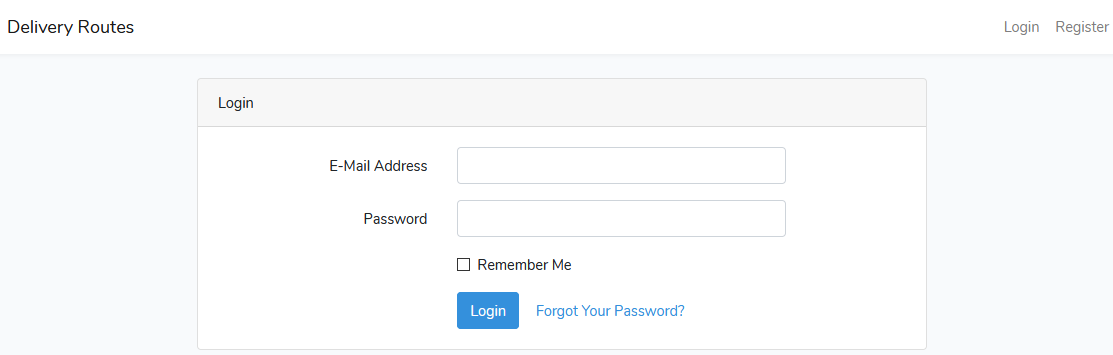
\includegraphics[width=0.4\textwidth]{./dados/figuras/fig7}
    \fonte{Autor}
    \label{fig:drLogin}
\end{figure}

%https://laravel.com/docs/5.7/hashing
O Laravel, juntamente com o Eloquent, disponibiliza a implementação de autenticação de maneira muito simples, por meio do comando \textit{php artisan make:auth}, onde, com poucas instruções e linhas de código, é possível montar a estrutura de cadastro de usuário, recuperação de senha e memória de sessão de maneira extremamente segura, devido ao algoritmo \textit{Bcrypt}
\footnote{Método de criptografia do tipo \textit{hash} adaptativo para senhas que apresenta uma segurança maior em relação à maioria dos outros métodos criptográficos por meio da implementação da variável “custo”, que é proporcional à quantidade de processamento necessária para criptografar a senha \cite{bcrypt}.}
, utilizado para realizar a criptografia da senha.

Ao realizar login, o administrador é apresentado à \textit{dashboard} do sistema, uma interface gráfica que fornece visualização fácil e rápida dos principais indicadores de desempenho, atualizados em tempo real, obtendo assim valores e médias relevantes sobre o processo de negócios. 

Destaca-se na \autoref{fig:drDashboard}, além de indicadores de: Pedidos Em Aberto, Pedidos Em Rota, Motoboys Disponíveis e Pedidos Concluídos, uma barra de menus contendo: Cadastros (Motoboys e Pagamentos) e Movimentos (Entregas e Pedidos Em Aberto).

\begin{figure}[H]
    \centering
    \caption{Delivery Routes - Dashboard}
    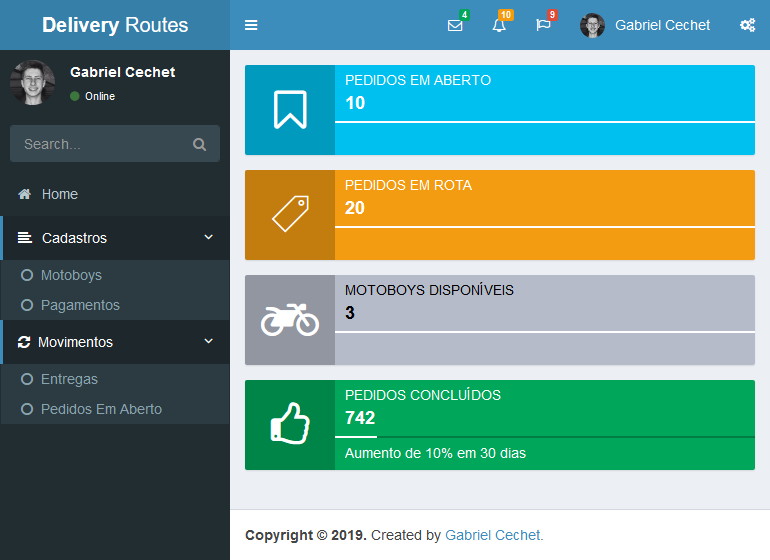
\includegraphics[width=1.0\textwidth]{./dados/figuras/fig13}
    \fonte{Autor}
    \label{fig:drDashboard}
\end{figure}

\newpage
Para desenvolver a \textit{dashboard}
%%% Rev-Madalozzo: listar todos os pacotes de terceiros AdminLTE e PDF


\newpage
\section{Coleta de dados}
\begin{figure}[H]
    \centering
    \caption{Delivery Routes - Coleta de dados}
    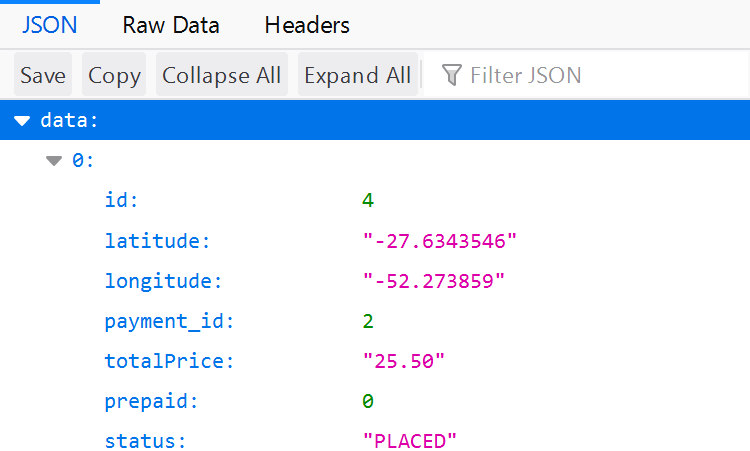
\includegraphics[width=0.6\textwidth]{./dados/figuras/fig14}
    \fonte{Autor}
    \label{fig:drPlacedAPI}
\end{figure}


\newpage
\section{Consulta de dados}
No momento em que a tela retratada na \autoref{fig:drAPIorder} inicia, um serviço de consulta para capturar informações do pedido requerido é executado. Esse serviço realiza uma requisição \textit{GET} na rota \textit{/order/\{id\}}, parametrizada para receber o código do pedido no estabelecimento, integrado pelo sistema anteriormente.

Nesse momento os possíveis status do pedido poderem ser: 
\\ \textit{INTEGRATED}, \textit{CANCELLED}, \textit{DISPATCHED}, \textit{DELIVERED} ou \textit{CONCLUDED}.

\begin{figure}[H]
    \centering
    \caption{Delivery Routes - API - order}
    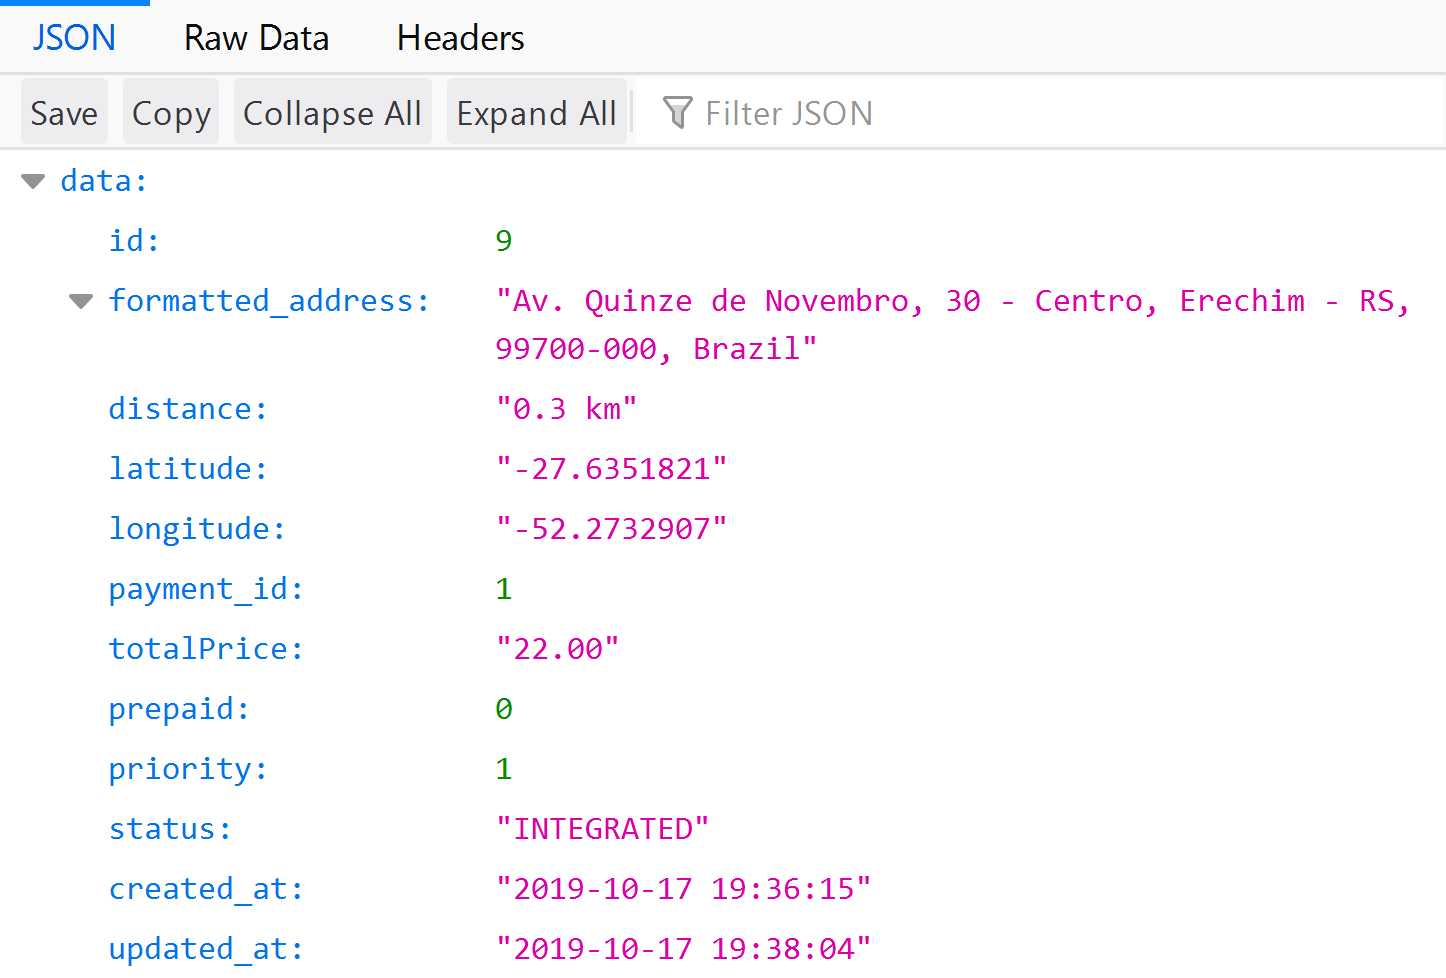
\includegraphics[width=0.9\textwidth]{./dados/figuras/fig22}
    \fonte{Autor}
    \label{fig:drAPIorder}
\end{figure}

Como resultado dessa consulta (como demonstra o \autoref{alg:getOrder}), o servidor retorna o objeto requisitado (em formato JSON) com os respectivos dados solicitados pela rota, por meio da ferramenta \textit{Resources}, exercendo a sua função como um camada de tratamento entre o Eloquent ORM e as respostas JSON que são expostas pela API. Essas classes, criadas ao executar o comando \textit{php artisan make:resource OrdersResource} através do Artisan, permitem transformar facilmente, \textit{models} e \textit{collections} em JSON.

\begin{lstlisting}[caption={Delivery Routes - Route order}, style=htmlcssjs, label=alg:getOrder]
Route::get('/order/{id}', function ($order_id) {
    return new OrdersResource(Order::find($order_id));
});
\end{lstlisting}

\newpage
\section{Módulo de entrega}
Neste módulo é apresentada a usabilidade do sistema por parte do motoboy, realizando a visualização da rota de entrega denominada para o momento.

\subsection{Tracking de entregas}
O primeiro status de uma entrega obrigatoriamente será \textit{CONFIRMED}, isso indica que a mesma foi planejada, visualizada e gerada pelo módulo de gerenciamento. Posteriormente a isso, a comanda (\autoref{fig:drCupom}) é impressa e então o fluxo de \textit{tracking} do pedido é iniciado (\autoref{fig:drFluxoPedido}).

 \begin{figure}[H]
    \centering
    \caption{Delivery Routes - Comanda do pedido}
    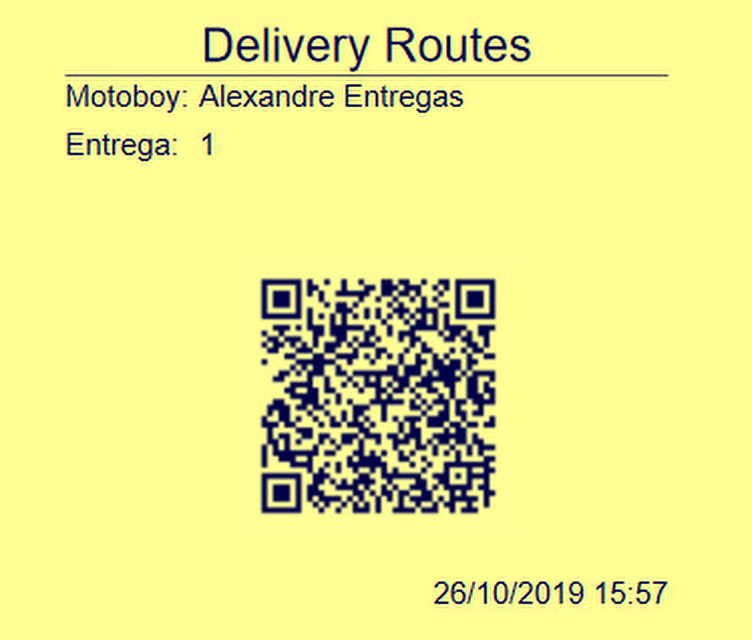
\includegraphics[width=0.4\textwidth]{./dados/figuras/fig24}
    \fonte{Autor}
    \label{fig:drCupom}
\end{figure}

\begin{figure}[H]
    \centering
    \caption{Delivery Routes - Fluxo do pedido}
    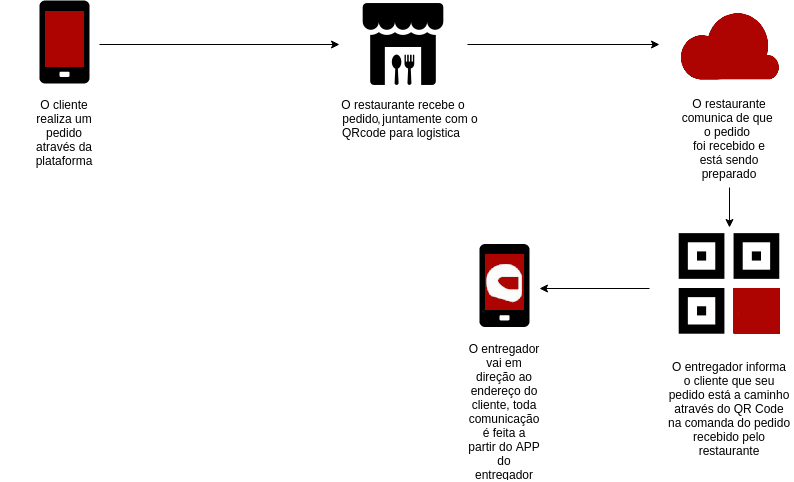
\includegraphics[width=0.85\textwidth]{./dados/figuras/fig25}
    \fonte{Adaptada de \citeonline{iFood}}
    \label{fig:drFluxoPedido}
\end{figure}

Neste cenário, ao ler o código QR impresso na comanda o motoboy é direcionado para a rota: \textit{/deliveries/{id}/dispatched} (\autoref{alg:funcDispatched}), alterando seu status para \textit{DISPATCHED} e executando uma nova rota: \textit{/deliveries/{id}/view}, onde o parâmetro solicitado para ambas é o código da entrega.

\begin{lstlisting}[caption={Delivery Routes - Função de despacho da entrega}, style=htmlcssjs, label=alg:funcDispatched]
public function dispatched($id) {
    $delivery = Delivery::find($id);
    $delivery->update(['status' => 'DISPATCHED']);
    return view('deliveries.view', compact('delivery'));
}
\end{lstlisting}

Logo após o despacho da entrega, é apresentada na tela no \textit{smartphone} do motoboy a representação, distância e tempo de deslocamento do percurso que deve ser percorrido na entrega desejada (\autoref{fig:drRotaEntregaInicio} e \autoref{fig:drRotaEntrega}).

\begin{figure}[H]
    \centering
    \caption{Delivery Routes - Despacho da entrega}
    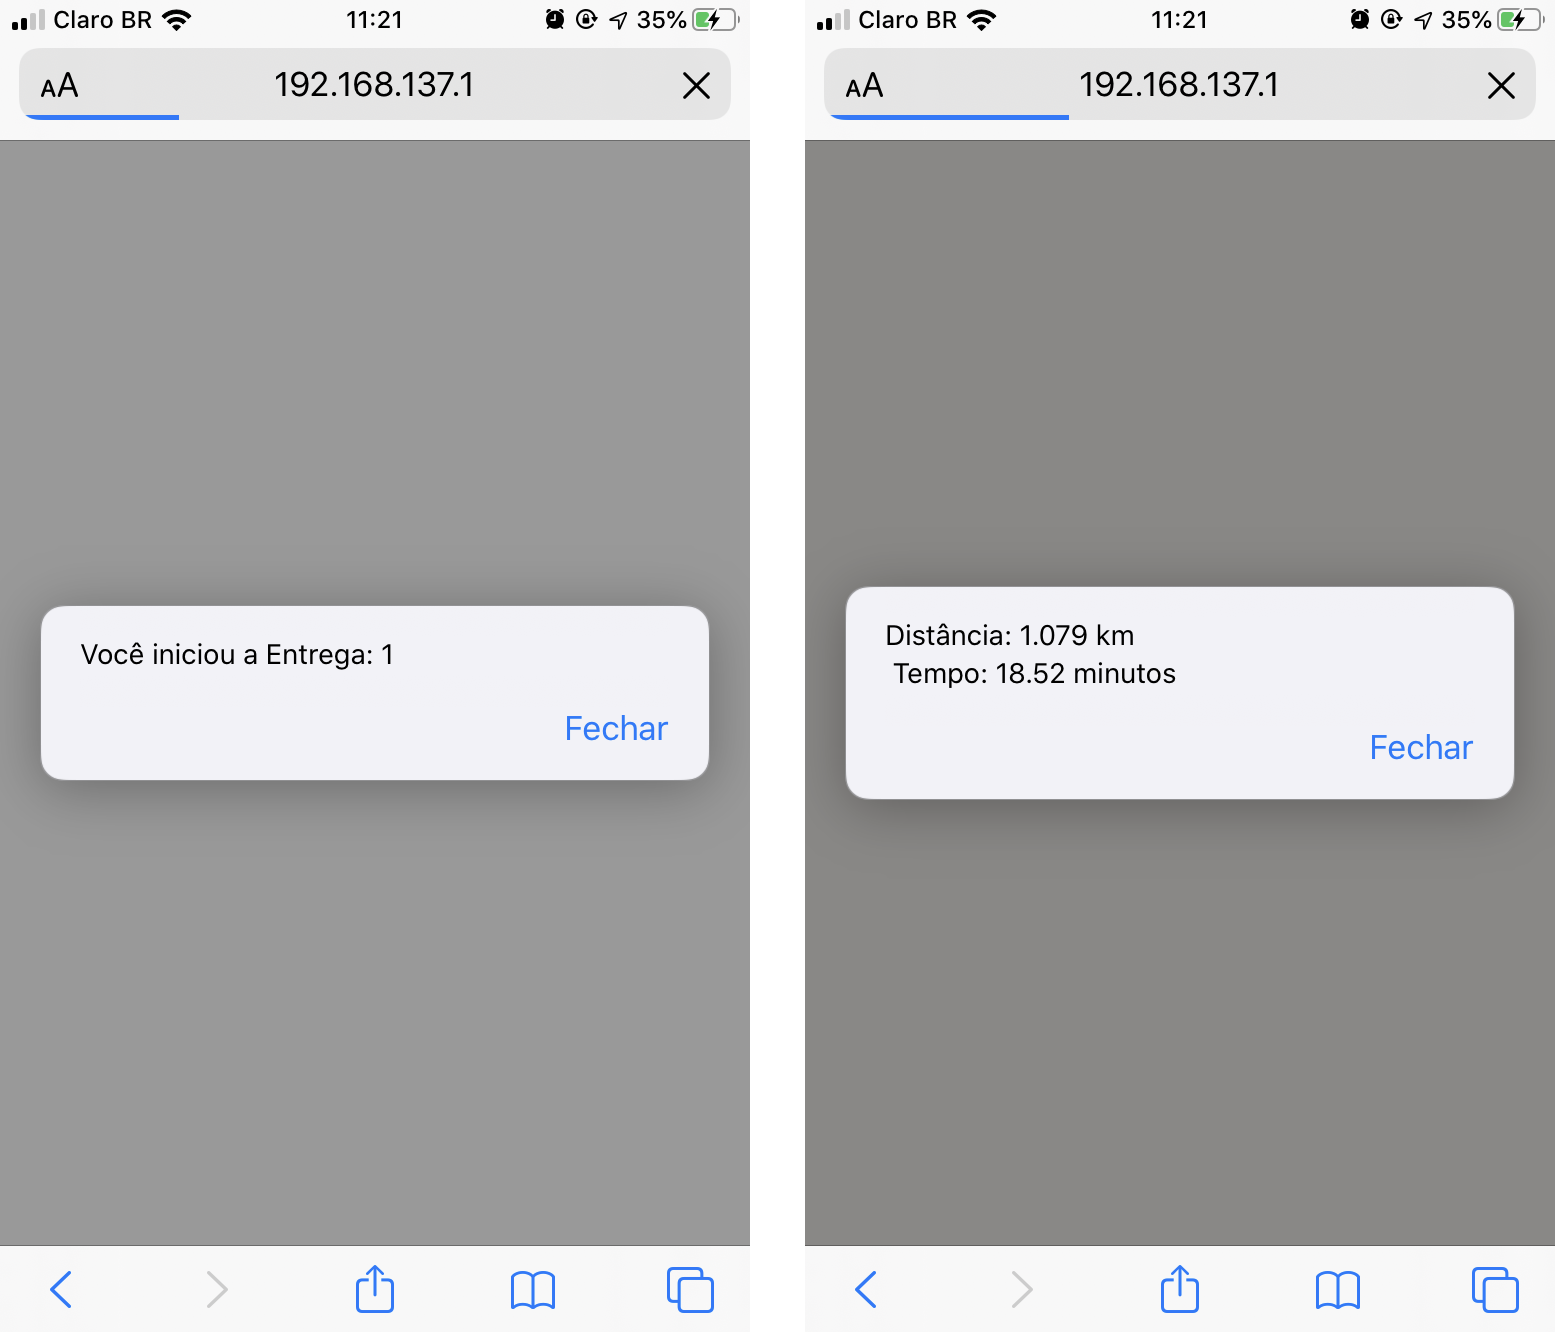
\includegraphics[width=0.9\textwidth]{./dados/figuras/fig28}
    \fonte{Autor}
    \label{fig:drRotaEntregaInicio}
\end{figure}

\newpage
\begin{figure}[H]
    \centering
    \caption{Delivery Routes - Mapa da entrega}
    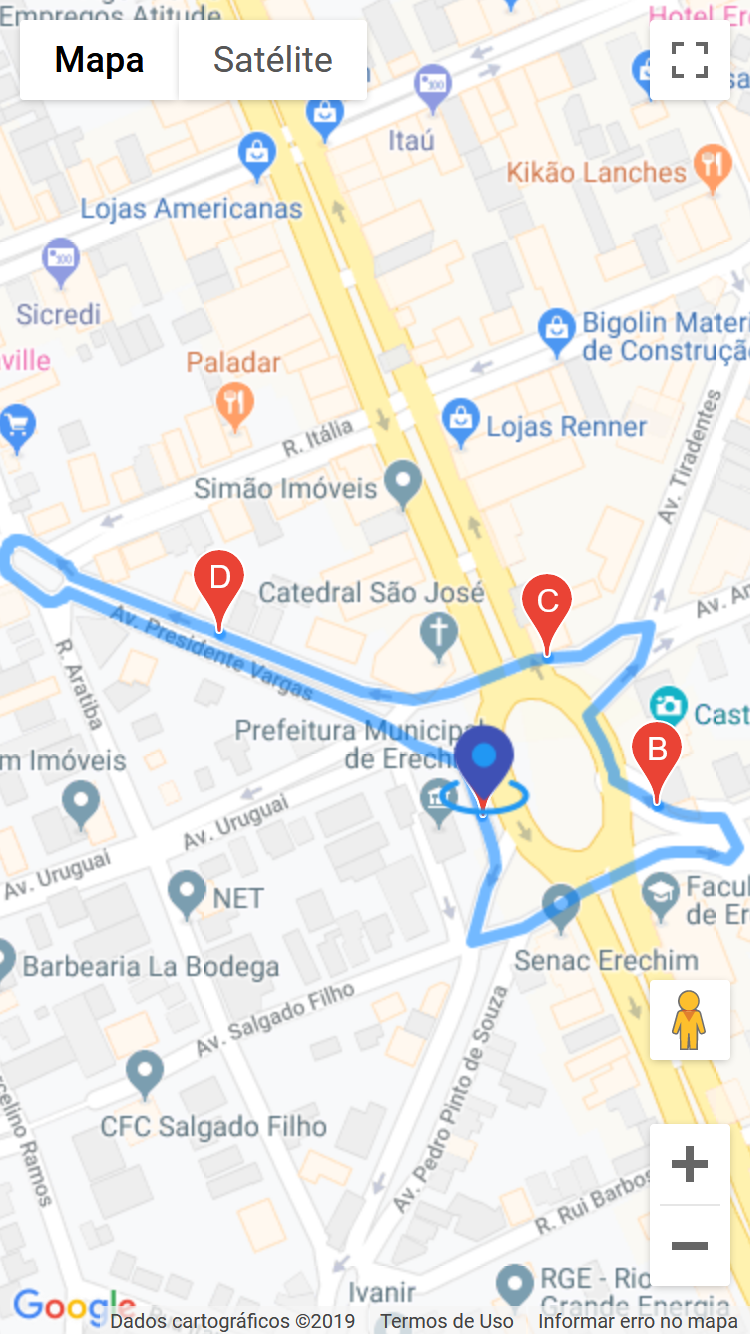
\includegraphics[width=0.8\textwidth]{./dados/figuras/fig27}
    \fonte{Autor}
    \label{fig:drRotaEntrega}
\end{figure}

\newpage
Para obter a rota entre dois pontos e exibi-la no mapa, é necessário utilizar o serviço da \textit{Google Directions} API. Lendo a sua documentação, verificou-se necessário a implementação das classes \textit{google.maps.DirectionsService} e o \textit{google.maps.DirectionsRenderer}.

Começando pelo \textit{DirectionsService}, o seu funcionamento é bem simples. Basta informar um objeto \textit{google.maps.DirectionsRequest}, o qual irá conter o ponto de origem e destino (\autoref{alg:currentPosition}), e o meio de transporte (carro, a pé, bicicleta ou transporte público), que ele irá retornar um objeto \textit{google.maps.DirectionsResult}, o qual contém as informações da rota, e o \textit{google.maps.DirectionsStatus}, que por sua vez define o estado final da requisição. Ele pode indicar sucesso (\textit{OK}), sem resultados (\textit{ZERO\_RESULTS}), erro (\textit{INVALID\_REQUEST} ou \textit{REQUEST\_DENIED}), etc.

\begin{lstlisting}[caption={Delivery Routes - Função de localização do usuário}, style=htmlcssjs, label=alg:currentPosition]
navigator.geolocation.getCurrentPosition(position);
function success(position) {
    currentPosition = new google.maps.LatLng(position.coords.latitude, position.coords.longitude);
};
\end{lstlisting}

Para adicionar os pontos de parada durante a rota, adquiridos através da rota: \textit{/delivering/{id}} (\autoref{alg:pedidosEntrega}), que retorna todos os pedidos da entrega solicitada, é preciso informar uma lista de objetos \textit{google.maps.DirectionsWaypoint} (\autoref{alg:waypoints}), que são alguns pontos pré-definidos no meio do trajeto no objeto \textit{DirectionsRequest} antes de passá-lo para o \textit{directionsService.route}.

\begin{lstlisting}[caption={Delivery Routes - Route pedidos da entrega}, style=htmlcssjs, label=alg:pedidosEntrega]
Route::get('/delivering/{id}', function ($delivery_id) {
    return new OrdersResource(DB::table('orders')
    ->leftJoin('deliveries_orders', 'orders.id', '=', 
    'deliveries_orders.order_id')
    ->where('deliveries_orders.delivery_id', $delivery_id)->get());
});
\end{lstlisting}

\begin{lstlisting}[caption={Delivery Routes - Preenchimento dos pontos de parada}, style=htmlcssjs, label=alg:waypoints]
$.getJSON(json, function(pontos) {
    $.each(pontos.data, function(index, ponto) {
        waypoints[position] = {
            'location': new google.maps.LatLng(ponto.latitude, ponto.longitude)
        };
    });
});
\end{lstlisting}

\newpage
Já o \textit{DirectionsRenderer}, basicamente, fica responsável por renderizar o resultado fornecido pelo \textit{DirectionsService} (\autoref{alg:directionsService}).

\begin{lstlisting}[caption={Delivery Routes - Requisição de renderização do mapa}, style=htmlcssjs, label=alg:directionsService]
var request = {
    origin: currentPosition,
    waypoints: waypoints,
    destination: currentPosition,
    travelMode: google.maps.TravelMode.DRIVING
};

directionsService.route(request, function(result, status) {
    if (status == google.maps.DirectionsStatus.OK) {
        directionsDisplay.setDirections(result);
    }
});
\end{lstlisting}

O cálculo de distância e tempo (\autoref{alg:computeTotalDistance}), exibido na \autoref{fig:drRotaEntregaInicio}, é a última etapa. Nele é computado o tempo de deslocamento entre os pontos e também o tempo dos trâmites de entrega do produto para o cliente final, estimado em 5 minutos cada.

\begin{lstlisting}[caption={Delivery Routes - Função de cálculo do deslocamento}, style=htmlcssjs, label=alg:computeTotalDistance]
function computeTotalDistance(result) {
    var totalDist = 0;
    var totalTime = -300; // retorno
    var myroute = result.routes[0];
    for (i = 0; i < myroute.legs.length; i++) {
        totalDist += myroute.legs[i].distance.value;
        totalTime += myroute.legs[i].duration.value;
        totalTime += 300;
    }
}
\end{lstlisting}

A maioria dos produtos da Google são pagos, porém há um crédito (200 dólares para uso mensal gratuito, que condizem com até 28 mil carregamentos no valor de 7 dólares por milhar) disponível no momento da requisição dos serviços, que vai sendo debitado na medida que é requisitado. Não é cobrado valor algum até que esse crédito seja totalmente utilizado. Ele pode ser usado no \textit{Maps}, no \textit{Routes} ou no \textit{Places}. Para fins de uso e cobrança, é necessário uma chave da API JavaScript do \textit{Google Maps}. A chave da API é um identificador exclusivo usado para autenticar solicitações associadas ao projeto.

%O trecho de código fonte que é apresentado a seguir demonstra como é o serviço de                login do aplicativo: 
%, conforme apresenta a figura 19 
%, conforme a figura 20 mostra
%% DESCRIÇÃO DA APLICAÇÃO-------------------------------------------------------------------

\chapter{DESCRIÇÃO DA APLICAÇÃO}

%% RESULTADOS-------------------------------------------------------------------

\chapter{ANÁLISE E DISCUSSÃO DOS RESULTADOS}

Cada capítulo deve conter uma pequena introdução (tipicamente, um ou dois parágrafos) que deve deixar claro o objetivo e o que será discutido no capítulo, bem como a organização do capítulo.
                    
%% ORIENTAÇÕES GERAIS------------------------------------------------------------


% SOBRE AS ILUSTRAÇÕES----------------------------------------------------------
\chapter{SOBRE AS ILUSTRAÇÕES}
\label{chap:apSobreIlust}

A seguir exemplifica-se como inserir ilustrações no corpo do trabalho. As ilustrações serão indexadas automaticamente em suas respectivas listas. A numeração sequencial de figuras, tabelas e equações também ocorre de modo automático.

Referências cruzadas são obtidas através dos comandos \verb|\label{}| e \verb|\ref{}|. Sendo assim, não é necessário por exemplo, saber que o número de certo capítulo é \ref{chap:fundamentacaoTeorica} para colocar o seu número no texto. Outra forma que pode ser utilizada é esta: \autoref{chap:fundamentacaoTeorica}, facilitando a inserção, remoção e manejo de elementos numerados no texto sem a necessidade de renumerar todos esses elementos.

% FIGURAS-----------------------------------------------------------------------
\chapter{FIGURAS}
\label{chap:figuras}

Exemplo de como inserir uma figura. A \autoref{fig:figura-exemplo1} aparece automaticamente na lista de figuras. Para saber mais sobre o uso de imagens no \LaTeX{} consulte literatura especializada \cite{Goossens2007}.

Os arquivos das figuras devem ser armazenados no diretório de "/dados".

\begin{figure}[!htb]
    \centering
    \caption{Exemplo de Figura}
    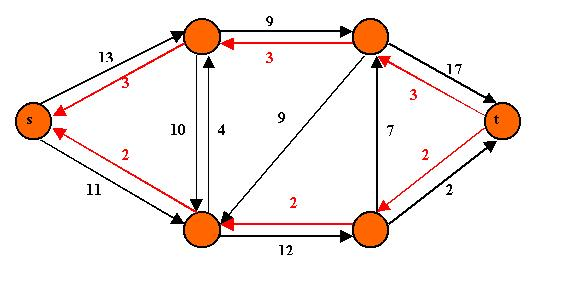
\includegraphics[width=0.5\textwidth]{./dados/figuras/figura1}
    \fonte{\citeonline{IRL2014}}
    \label{fig:figura-exemplo1}
\end{figure}

% QUADROS E TABELAS---------------------------------------------------------------
\chapter{QUADROS E TABELAS}
\label{chap:tabelas}

Exemplo de como inserir o \autoref{qua:quadro-exemplo1} e a \autoref{tab:tabela-exemplo1}. Ambos aparecem automaticamente nas suas respectivas listas. Para saber mais informações sobre a construção de tabelas no \LaTeX{} consulte literatura especializada \cite{Mittelbach2004}.

Ambos os elementos (Quadros e Tabelas) devem ser criados em arquivos separados para facilitar manutenção e armazenados no diretório de "/dados".

\begin{quadro}[!htb]
    \centering
    \caption{Exemplo de Quadro.\label{qua:quadro-exemplo1}}
    \begin{tabular}{|p{7cm}|p{7cm}|}
        \hline
        \textbf{BD Relacionais} & \textbf{BD Orientados a Objetos} \\
        \hline
        Os dados são passivos, ou seja, certas operações limitadas podem ser automaticamente acionadas quando os dados são usados. Os dados são ativos, ou seja, as solicitações fazem com que os objetos executem seus métodos. & Os processos que usam dados mudam constantemente. \\
        \hline
    \end{tabular}
    \fonte{\citeonline{Barbosa2004}}
\end{quadro}


A diferença entre quadro e tabela está no fato que um quadro é formado por linhas horizontais e verticais. Deve ser utilizado quando o conteúdo é majoritariamente não-numérico. O número do quadro e o título vem acima do quadro, e a fonte, deve vir abaixo. E Uma tabela é formada apenas por linhas verticais. Deve ser utilizada quando o conteúdo é majoritariamente numérico. O número da tabela e o título vem acima da tabela, e a fonte, deve vir abaixo, tal como no quadro.

\begin{table}[!htb]
    \centering
    \caption[Resultado dos testes]{Resultado dos testes.
    \label{tab:tabela-exemplo1}}
    \begin{tabular}{rrrrr}
        \toprule
            & Valores 1 & Valores 2 & Valores 3 & Valores 4 \\
        \midrule
            Caso 1 & 0,86 & 0,77 & 0,81 & 163 \\
            Caso 2 & 0,19 & 0,74 & 0,25 & 180 \\
            Caso 3 & 1,00 & 1,00 & 1,00 & 170 \\
        \bottomrule
    \end{tabular}
    \fonte{\citeonline{Barbosa2004}}
\end{table}


%CRONOGRAMA PARA PROJETO-----------------------------------------------------------------------
% Exemplo de quadro para planejamento de projeto de pesquisa
% \chapter{PLANEJAMENTO DO TRABALHO}
% \label{sec:planejamento}
% Planejamento do Trabalho----------------------------------------------------------------
% Esta seção não precisa ser editada, apenas edite o quadro 1 armazenada no diretório ".\dados\quadros"
% O planejamento do trabalho de estágio que será desenvolvido pelo aluno, ao longo do período letivo, está descrito no cronograma do Quadro 2. Neste cronograma constam todas as atividades com seus respectivos prazos para o cumprimento.
% \begin{quadro}[!htb]
    %\centering
    \caption{Cronograma de Atividades.\label{qua:quadro1}}
    \begin{tabular}{|p{4.5cm}|p{0.7cm}|p{0.7cm}|p{0.7cm}|p{0.7cm}|p{0.7cm}|p{0.7cm}|p{0.7cm}|p{0.7cm}|p{0.7cm}|p{0.7cm}|}
        \hline
        \textbf{Atividades} & \textbf{Mar} & \textbf{Abr} & \textbf{Mai} & \textbf{Jun} & \textbf{Jul} & \textbf{Ago} & \textbf{Set} & \textbf{Out} & \textbf{Nov} & \textbf{Dez} \\
        \hline
        \small{1. Revisão dos apontamentos da banca} &   &   &   &   &   &   &   &   &   &  \\
        \hline
        \small{2. Revisão bibliográfica} &   &   &   &   &   &   &   &   &   &  \\
        \hline
	\small{3. Redação do projeto de TCC} &   &   & X & X &   &   &   &   &   &  \\
        \hline
	\small{4. Defesa do projeto de TCC} &   &   &   &   & X &   &   &   &   &  \\
        \hline
	\small{5. Escrita da Monografia de TCC} &   &   &   &   &   & X & X  & X &   &  \\
        \hline
	\small{6. Elaboração da apresentação final} &   &   &   &   &   &   &   & X & X &  \\
        \hline
	\small{7. Defesa final do TCC} &   &   &   &   &   &   &   &   & X &  \\
        \hline
    \end{tabular}
\end{quadro}
%-----------------------------------------------------------------------------------------

% EQUAÇÕES-----------------------------------------------------------------------
\chapter{EQUAÇÕES}
\label{chap:equacoes}

Exemplo de como inserir a \autoref{eq:equacao-exemplo1} e a Eq. \ref{eq:equacao-exemplo2} no corpo do texto \footnote{Deve-se atentar ao fato de a formatação das equações ficar muito boa esteticamente.}. Observe que foram utilizadas duas formas distintas para referenciar as equações.

\begin{equation}
    X(s) = \int\limits_{t = -\infty}^{\infty} x(t) \, \text{e}^{-st} \, dt
    \label{eq:equacao-exemplo1}
\end{equation}

\begin{equation}
    F(u, v) = \sum_{m = 0}^{M - 1} \sum_{n = 0}^{N - 1} f(m, n) \exp \left[ -j 2 \pi \left( \frac{u m}{M} + \frac{v n}{N} \right) \right]
    \label{eq:equacao-exemplo2}
\end{equation}

% ALGORITMOS-----------------------------------------------------------------------
\chapter{ALGORITMOS}
\label{chap:algoritmos}

Exemplo de como inserir um algoritmo. Para inserção de algoritmos utiliza-se o pacote {\ttfamily algorithm2e} que já está devidamente configurado dentro do template.

Os algoritmos devem ser criados em arquivos separados para facilitar manutenção e armazenados no diretório de "/dados".\\
\\

\begin{algorithm}
    \caption{Exemplo de Algoritmo}
    \KwIn{o número $n$ de vértices a remover, grafo original $G(V, E)$}
    \KwOut{grafo reduzido $G'(V,E)$}
    $removidos \leftarrow 0$ \\
    \While {removidos $<$ n } {
        $v \leftarrow$ Random$(1, ..., k) \in V$ \\
            \For {$u \in adjacentes(v)$} {
                remove aresta (u, v)\\
                $removidos \leftarrow removidos + 1$\\
            }
            \If {há  componentes desconectados} {
                remove os componentes desconectados\\
            }
        }
\end{algorithm}


% SOBRE AS LISTAS--------------------------------------------------------------------
\chapter{SOBRE AS LISTAS}
\label{chap:apSobreLista}

Para construir listas de "\textit{bullets}"{} ou listas enumeradas, inclusive listas aninhadas, é utilizado o pacote \verb|paralist|.

Exemplo de duas listas não numeradas aninhadas, utilizando o comando \verb|\itemize|. Observe a indentação, bem como a mudança automática do tipo de "\textit{bullet}"{} nas listas aninhadas.

\begin{itemize}
    \item item não numerado 1
    \item item não numerado 2
    \begin{itemize}
        \item subitem não numerado 1
        \item subitem não numerado 2
        \item subitem não numerado 3
    \end{itemize}
    \item item não numerado 3
\end{itemize}

Exemplo de duas listas numeradas aninhadas, utilizando o comando \verb|\enumerate|. Observe a numeração progressiva e indentação das listas aninhadas.

\begin{enumerate}
    \item item numerado 1
    \item item numerado 2
    \begin{enumerate}
        \item subitem numerado 1
        \item subitem numerado 2
        \item subitem numerado 3
    \end{enumerate}
    \item item numerado 3
\end{enumerate}

% SOBRE AS CITAÇÕES E CHAMADAS DE REFERÊNCAS----------------------------------------------
\chapter{SOBRE AS CITAÇÕES E CHAMADAS DE REFERÊNCAS}
\label{chap:apSobreCita}

Citações são trechos de texto ou informações obtidas de materiais consultadss quando da elaboração do trabalho. São utilizadas no texto com o propósito de esclarecer, completar e embasar as ideias do autor. Todas as publicações consultadas e utilizadas (por meio de citações) devem ser listadas, obrigatoriamente, nas referências bibliográficas, para preservar os direitos autorais. São classificadas em citações indiretas e diretas.

% CITAÇÕES INDIRETAS-----------------------------------------------------------------------
\chapter{CITAÇÕES INDIRETAS}
\label{chap:citacoesLivres}

É a transcrição, com suas próprias palavras, das idéias de um autor, mantendo-se o sentido original. A citação indireta é a maneira que o pesquisador tem de ler, compreender e gerar conhecimento a partir do conhecimento de outros autores. Quanto à chamada da referência, ela pode ser feita de duas maneiras distintas, conforme o nome do(s) autor(es) façam parte do seu texto ou não. Exemplo de chamada fazendo parte do texto:\\
\\Enquanto \citeonline{Maturana2003} defendem uma epistemologia baseada na biologia. Para os autores, é necessário rever \ldots.\\

A chamada de referência foi feita com o comando \verb|\citeonline{chave}|, que produzirá a formatação correta.

A segunda forma de fazer uma chamada de referência deve ser utilizada quando se quer evitar uma interrupção na sequência do texto, o que poderia, eventualmente, prejudicar a leitura. Assim, a citação é feita e imediatamente após a obra referenciada deve ser colocada entre parênteses. Porém, neste caso específico, o nome do autor deve vir em caixa alta, seguido do ano da publicação. Exemplo de chamada não fazendo parte do texto:\\
\\Há defensores da epistemologia baseada na biologia que argumentam em favor da necessidade de \ldots \cite{Maturana2003}.\\

Nesse caso a chamada de referência deve ser feita com o comando \verb|\cite{chave}|, que produzirá a formatação correta.

% CITAÇÕES DIRETAS-----------------------------------------------------------------------
\chapter{CITAÇÕES DIRETAS}
\label{chap:citacoesLiterais}

É a transcrição ou cópia de um parágrafo, de uma frase, de parte dela ou de uma expressão, usando exatamente as mesmas palavras adotadas pelo autor do trabalho consultado.

Quanto à chamada da referência, ela pode ser feita de qualquer das duas maneiras já mencionadas nas citações indiretas, conforme o nome do(s) autor(es) façam parte do texto ou não. Há duas maneiras distintas de se fazer uma citação direta, conforme o trecho citado seja longo ou curto.

Quando o trecho citado é longo (4 ou mais linhas) deve-se usar um parágrafo específico para a citação, na forma de um texto recuado (4 cm da margem esquerda), com tamanho de letra menor e espaçamento entrelinhas simples. Exemplo de citação longa:
\\\begin{citacao}
    Desse modo, opera-se uma ruptura decisiva entre a reflexividade filosófica, isto é a possibilidade do sujeito de pensar e de refletir, e a objetividade científica. Encontramo-nos num ponto em que o conhecimento científico está sem consciência. Sem consciência moral, sem consciência reflexiva e também subjetiva. Cada vez mais o desenvolvimento extraordinário do conhecimento científico vai tornar menos praticável a própria possibilidade de reflexão do sujeito sobre a sua pesquisa \cite[p.~28]{Silva2000}.
\end{citacao}

Para fazer a citação longa deve-se utilizar os seguintes comandos:
\begin{verbatim}
\begin{citacao}
<texto da citacao>
\end{citacao}
\end{verbatim}

No exemplo acima, para a chamada da referência o comando \verb|\cite[p.~28]{Silva2000}| foi utilizado, visto que os nomes dos autores não são parte do trecho citado. É necessário também indicar o número da página da obra citada que contém o trecho citado.

Quando o trecho citado é curto (3 ou menos linhas) ele deve inserido diretamente no texto entre aspas. Exemplos de citação curta:\\
\\A epistemologia baseada na biologia parte do princípio de que "assumo que não posso fazer referência a entidades independentes de mim para construir meu explicar" \cite[p.~35]{Maturana2003}.\\
\\A epistemologia baseada na biologia de \citeonline[p.~35]{Maturana2003} parte do princípio de que "assumo que não posso fazer referência a entidades independentes de mim para construir meu explicar".

% DETALHES SOBRE AS CHAMADAS DE REFERÊNCIAS---------------------------------------------------------
\chapter{DETALHES SOBRE AS CHAMADAS DE REFERÊNCIAS}
\label{chap:referUtilizadas}

Outros exemplos de comandos para as chamadas de referências e o resultado produzido por estes:\\
\\\citeonline{Maturana2003} \ \ \  \verb|\citeonline{Maturana2003}|\\
\citeonline{Barbosa2004} \ \ \   \verb|\citeonline{Barbosa2004}|\\
\cite[p.~28]{Silva2000} \ \ \  \verb|\cite[p.~28]{Silva2000}|\\
\citeonline[p.~33]{Silva2000} \ \ \   \verb|\citeonline[p.~33]{v}|\\
\cite[p.~35]{Maturana2003} \ \ \   \verb|\cite[p.~35]{Maturana2003}|\\
\citeonline[p.~35]{Maturana2003} \ \ \   \verb|\citeonline[p.~35]{Maturana2003}|\\
\cite{Barbosa2004,Maturana2003} \ \ \   \verb|\cite{Barbosa2004,Maturana2003}|\\

% SOBRE AS REFERÊNCIAS BIBLIOGRÁFICAS-------------------------------------------------------
\chapter{SOBRE AS REFERÊNCIAS BIBLIOGRÁFICAS}
\label{chap:apSobreRefer}

A bibliografia é feita no padrão \textsc{Bib}\TeX{}. As referências são colocadas em um arquivo separado. Neste template as referências são armazenadas no arquivo "base-referencias.bib".

Existem diversas categorias documentos e materiais componentes da bibliografia. A classe abn\TeX{} define as seguintes categorias (entradas):

\begin{verbatim}
@book
@inbook
@article
@phdthesis
@mastersthesis
@monography
@techreport
@manual
@proceedings
@inproceedings
@journalpart
@booklet
@patent
@unpublished
@misc
\end{verbatim}

Cada categoria (entrada) é formatada pelo pacote \citeonline{abnTeX22014d} de uma forma específica. Algumas entradas foram introduzidas especificamente para atender à norma \citeonline{NBR6023:2002}, são elas: \verb|@monography|, \verb|@journalpart|,\verb|@patent|. As demais entradas são padrão \textsc{Bib}\TeX{}. Para maiores detalhes, refira-se a \citeonline{abnTeX22014d}, \citeonline{abnTeX22014b}, \citeonline{abnTeX22014c}.

% NOTAS DE RODAPÉ--------------------------------------------------------------------------
\chapter{NOTAS DE RODAPÉ}
\label{chap:notasRodape}

As notas de rodapé pode ser classificadas em duas categorias: notas explicativas\footnote{é o tipo mais comum de notas que destacam, explicam e/ou complementam o que foi dito no corpo do texto, como esta nota de rodapé, por exemplo.} e notas de referências. A notas de referências, como o próprio nome ja indica, são utilizadas para colocar referências e/ou chamadas de referências sob certas condições.
                   
% CONCLUSÃO--------------------------------------------------------------------

\chapter{CONCLUSÃO E TRABALHOS FUTUROS}

\postextual
% INSERE ELEMENTOS PÓS-TEXTUAIS
% REFERÊNCIAS------------------------------------------------------------------

% Carrega o arquivo "exemplo-referencias.bib" e extrai automaticamente as referências citadas
{\renewcommand{\contentsname}{MAC}}
\bibliography{./referencias}
\bibliographystyle{abntex2-alf} % Define o estilo ABNT para formatar a lista de referências
% OBSERVAÇÕES------------------------------------------------------------------
% Este arquivo não precisa ser alterado.
% APÊNDICES--------------------------------------------------------------------

\begin{apendicesenv}
\partapendices

% Primeiro apêndice------------------------------------------------------------
\chapter{Diagrama de Classes}
\label{chap:apendiceA}

\begin{figure}[H]
    \centering
    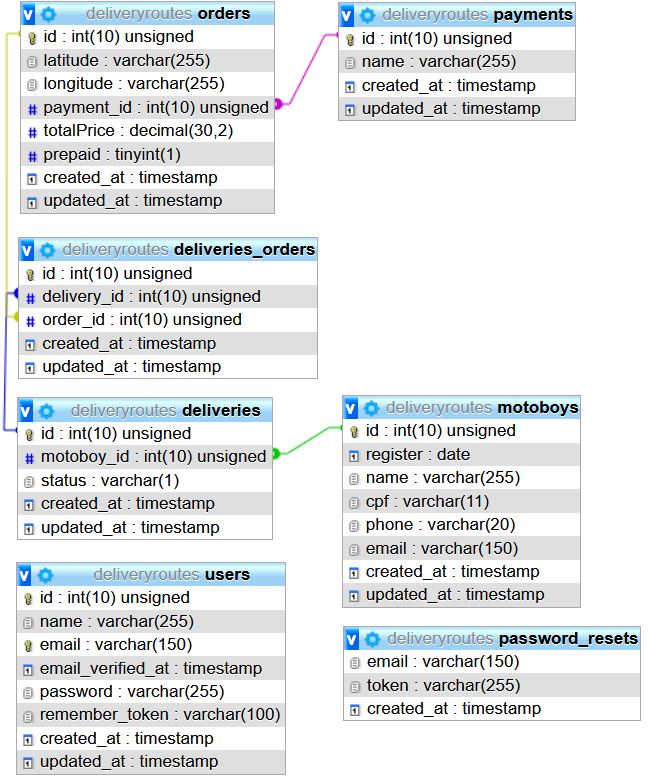
\includegraphics[width=0.9\textwidth]{./dados/figuras/apendiceA}
\end{figure}

\end{apendicesenv}

%% ANEXO------------------------------------------------------------------------

\begin{anexosenv}
\partanexos

% Primeiro anexo---------------------------------------------------------------
\chapter{Nome do anexo}     % edite para alterar o título deste anexo
\label{chap:anexoA}

Lembre-se que a diferença entre apêndice e anexo diz respeito à autoria do texto e/ou material ali colocado.

Caso o material ou texto suplementar ou complementar seja de sua autoria, então ele deverá ser colocado como um apêndice. Porém, caso a autoria seja de terceiros, então o material ou texto deverá ser colocado como anexo.

Caso seja conveniente, podem ser criados outros anexos para o seu trabalho acadêmico. Basta recortar e colar este trecho neste mesmo documento. Lembre-se de alterar o "label"{} do anexo.

Organize seus anexos de modo a que, em cada um deles, haja um único tipo de conteúdo. Isso facilita a leitura e compreensão para o leitor do trabalho. É para ele que você escreve.

% Novo anexo-------------------------------------------------------------------
\chapter{Nome do outro anexo}
\label{chap:anexoB}

conteúdo do outro anexo

\end{anexosenv}


\end{document}
